\documentclass[11pt]{article}

\usepackage{CJKutf8} % For Chinese support
\usepackage{acl}

% Standard packages
\usepackage{latexsym}
\usepackage[T1]{fontenc}
\usepackage[utf8]{inputenc}
%\usepackage{microtype}
\usepackage{inconsolata}
\usepackage{graphicx}
\usepackage{amsmath}
\usepackage{amssymb}
\usepackage{array}
\usepackage{booktabs}
\usepackage{multirow}
\usepackage{xcolor}
\usepackage{algorithm}
\usepackage{algorithmic}
\usepackage{url}
\usepackage{tikz}
\usetikzlibrary{shapes.geometric, arrows.meta, positioning, fit, backgrounds, calc}
\usepackage{pgfplots}
\pgfplotsset{compat=1.16}
\usepackage{tcolorbox}
\usepackage{enumitem}
\setlist{noitemsep, topsep=2pt, parsep=1pt, partopsep=0pt}
\setlength{\textfloatsep}{8pt plus 1.0pt minus 2.0pt}
\setlength{\floatsep}{8pt plus 1.0pt minus 2.0pt}
\setlength{\intextsep}{8pt plus 1.0pt minus 2.0pt}
\newcolumntype{L}[1]{>{\raggedright\arraybackslash}p{#1}}
\newcolumntype{C}[1]{>{\centering\arraybackslash}p{#1}}

\title{PersonaForge: Psychology-Grounded Dual-Process Architecture \\ for Personality-Consistent Role-Playing Agents}

\author{
  Jizhou Tong$^{\dagger \ast}$ \\
  Wuhan University \\
  \texttt{fqwqf6@whu.edu.cn}
  \And
  Sirui Zou$^{\dagger}$ \\
  Southwestern University of Finance and Economics \\
  \texttt{siruizou2005@gmail.com}
}

\begin{document}
\begin{CJK*}{UTF8}{gbsn}
\maketitle
\begingroup
\renewcommand{\thefootnote}{}
\footnotetext{$^{\dagger}$Equal contribution.\quad $^{\ast}$Corresponding author.}
\endgroup

\begin{abstract}
Large Language Models excel at role-playing but struggle to maintain consistent personalities across \textit{extended multi-turn interactions}. We propose \textbf{PersonaForge}, combining \textbf{(1) a three-layer personality architecture} grounded in psychological theory and \textbf{(2) a dual-process generation mechanism} inspired by cognitive science. We test two falsifiable claims: \textbf{Claim 1 (Orthogonality)}: Psychology-grounded dimensions (Big Five + Defense Mechanisms) provide more orthogonal constraints than natural language descriptions, reducing long-dialogue drift. \textbf{Claim 2 (Integration Necessity)}: High-dimensional personality constraints create ``production interference'' requiring a cognitive workspace (Inner Monologue) to resolve---removing it degrades performance \textit{below} simpler baselines. Experiments on \textbf{88 characters} demonstrate: (1) +19.4\% personality consistency (PC) over the Structured-CoT baseline, with human correlation $r=0.82$, (2) reduced drift over 50-turn conversations (6.3\% vs. 24.8\% baseline), and (3) +64.7\% defense mechanism manifestation. External validation on \textbf{RoleBench} confirms generalization (73.2\% win-rate, drift 8.4\% vs. 20.4\%). Selective dual-process activation achieves 96\% of full-system performance with only \textbf{13.4\% token overhead}. Human evaluation confirms more authentic and psychologically coherent character behaviors. Code and data: \url{https://github.com/fQwQf/PersonaForge}.
\end{abstract}

\section{Introduction}

Role-playing with Large Language Models (LLMs) has emerged as a compelling application, enabling immersive storytelling and virtual companionship \citep{chen2024persona}. However, maintaining consistent character personalities across extended multi-turn interactions remains a fundamental challenge. Current approaches often suffer from:

\begin{enumerate}
    \item \textbf{Character drift}: Personality traits gradually shift or become inconsistent over long conversations
    \item \textbf{Shallow personality modeling}: Reliance on surface-level text descriptions without psychological grounding
    \item \textbf{Style instability}: Language patterns fluctuate based on prompt variations
    \item \textbf{Static representations}: Inability to model dynamic emotional states
\end{enumerate}

To address these limitations, we propose \textbf{PersonaForge}, a framework integrating personality psychology and cognitive science. Our key insight is that \textbf{different aspects of personality collapse require different architectural solutions}---no single mechanism suffices. To address internal conflicts to achieve psychological integration, our architecture explicitly models both conscious expression and the suppressed cognitive processes beneath. To our knowledge, this is \textbf{among the first computational frameworks} to operationalize Vaillant's defense mechanisms within LLM agents as programmable cognitive strategies.

\paragraph{SFT Enhancer and Inference-Time Guardrail.} While SFT achieves stylistic mimicry \citep{shao2023character}, \textbf{low-resource SFT} (typical in cold-start scenarios) often captures the ``surface voice'' without the ``cognitive core,'' leading to rigidity in long contexts. PersonaForge can serve as an \textbf{Inference-time Guardrail} or \textbf{SFT Enhancer}: even effectively fine-tuned models benefit from our dual-process architecture to maintain consistency under stress. Furthermore, our approach solves the \textbf{cold-start problem} through \textbf{Automated Parameter Acquisition}: users need only provide raw text (e.g., a Wiki link), from which our pipeline extracts the Big Five and Defense Mechanism parameters, enabling high-fidelity role-play without training.

\begin{figure}[t]
\centering
\begin{tcolorbox}[colback=gray!10, colframe=black!70, title=\textbf{Case Study: Psychological Defense Mechanism (Tyrion Lannister)}]
\small
\textbf{Context}: Tywin Lannister calls Tyrion a "disgrace" to the family.

\medskip
\textbf{SFT Baseline (template-locked)}: \\
"I suppose I should be offended, but then again, I've always been a bit of a disappointment..." \\
\textit{Analysis}: Acknowledges insult but lacks the characteristic wit. \textcolor{red}{\textbf{Psychologically Flat}}.

\medskip
\textbf{Ours (With Humor Defense)}: \\
\textit{Inner Monologue}: [Defense: Humor $\rightarrow$ "Imagine him in a gilded bathtub..."] \\
\textit{Response}: "Imagine him, in a gilded bathtub filled with rose petals, sipping champagne and humming a jaunty tune—quite the spectacle, wouldn't you say? Shall we raise a glass to my father?" \\
\textit{Analysis}: Deflects the ego-threat by reducing the aggressor to absurdity. \textcolor{blue}{\textbf{Psychologically Authentic}}.
\end{tcolorbox}
\caption{Impact of Defense Mechanisms. The architecture enables characters to \textit{face their true selves}, transforming generic emotional reactions into character-specific coping strategies.}
\label{fig:motivating}
\end{figure}

Our contributions:

\paragraph{Two Testable Research Claims.} We frame our design around two falsifiable claims: \textbf{(1) The Orthogonality Hypothesis}---psychology-grounded dimensions (Big Five + Defense Mechanisms) provide more orthogonal constraints than natural language descriptions. Evidence: ``Generic Structured'' ablation (Table~\ref{tab:ablation}) shows $\Delta$PC = -0.18 when replacing Big Five/DM with natural language. \textbf{(2) The Integration Necessity Hypothesis}---high constraint density causes ``production interference'' without a cognitive workspace. Evidence: ``w/o Dual-Process'' achieves PC 0.57 vs. Structured-CoT's 0.72, confirming the three-layer profile \textit{requires} the Inner Monologue.

\paragraph{Why Defense Mechanisms Are Not ``Situation Templates.''} DMs are \textbf{cognitive distortion procedures}, not behavioral scripts---they specify \textit{how to perceive} stressors, not just \textit{what to say}. The same DM produces radically different outputs depending on stressor content. Ablation shows DM removal degrades \textit{activation precision} from 92\% to 61\%. We model DMs as \textit{pre-conscious cognitive routines} \citep{vaillant1994ego}---the Inner Monologue represents what surfaces to working memory, not the unconscious process itself. Following Marr's levels, we implement an \textit{algorithmic} approximation of a \textit{computational} theory of personality.

\paragraph{Three-Layer Personality Architecture.} We introduce a \textbf{functionally decomposed} architecture: \textbf{Core Traits} (Big Five + Defense Mechanisms) prevent \textit{trait drift}; \textbf{Speaking Style Matrix} prevents \textit{style collapse}; \textbf{Dynamic State} prevents \textit{context blindness} by tracking emotional/relational evolution. Inspired by Kahneman's dual-system theory \citep{kahneman2011thinking}, we implement \textit{Think-then-Speak} that activates only for critical interactions ($\approx$40\% of turns), achieving 96\% of full dual-process performance at 89\% cost.

\paragraph{Rigorous Validation.} We address LLM-as-Judge concerns through: (1) \textbf{High-Load Long-Dialogue Benchmark} (50 turns), (2) \textbf{Human Expert Validation} ($r = 0.82$), (3) \textbf{Cross-Generator Ranking Consistency}, and (4) \textbf{External Validation on RoleBench} \citep{wang2024rolellm}: 73.2\% pairwise win-rate with drift reduced from 20.4\% to 8.4\%. Our architecture is \textbf{model-agnostic}: a fully open-source pipeline using DeepSeek-V3 achieves PC 0.84.


\section{Related Work}

\paragraph{LLM-Based Role-Playing and Dialogue Systems.}
Recent work explores character-consistent generation through fine-tuning \citep{shao2023character}, retrieval-augmented generation \citep{wang2024rolellm}, and psychological interviews \citep{wang2024incharacter}. Persona-conditioned dialogue \citep{zhang2018personalizing} and memory-augmented agents \citep{packer2023memgpt,park2023generative} enable long-context management but lack deep personality structuring. Our structured Big Five + DM representations provide orthogonal constraints that reduce long-dialogue drift.

\paragraph{Personality Modeling and Dual-Process Reasoning.}
The Big Five model and Vaillant's defense mechanisms have been applied to NLP tasks \citep{zhong2020towards}, but prior work rarely integrates DMs as programmable cognitive strategies. Kahneman's dual-system theory \citep{kahneman2011thinking} inspired chain-of-thought \citep{wei2022chain} and ReAct \citep{yao2022react}. Critically, \citet{feng2025reasoning} show naive reasoning harms role-playing; RAR \citep{tang2025thinking} addresses style preservation; PersonaForge tackles context-conditional cognitive processing. CharacterBox \citep{wang2025characterbox} and trajectory-based assessment \citep{tan2025detecting} provide complementary long-horizon evaluation approaches.


\section{Methodology}

We propose a \textbf{Functionally Decomposed Architecture}, creating a modular system where distinct psychological dimensions are handled by specialized components rather than a monolithic prompt. This decomposition allows for targeted intervention and ablation.

\begin{figure*}[t]
\centering
\resizebox{\linewidth}{!}{
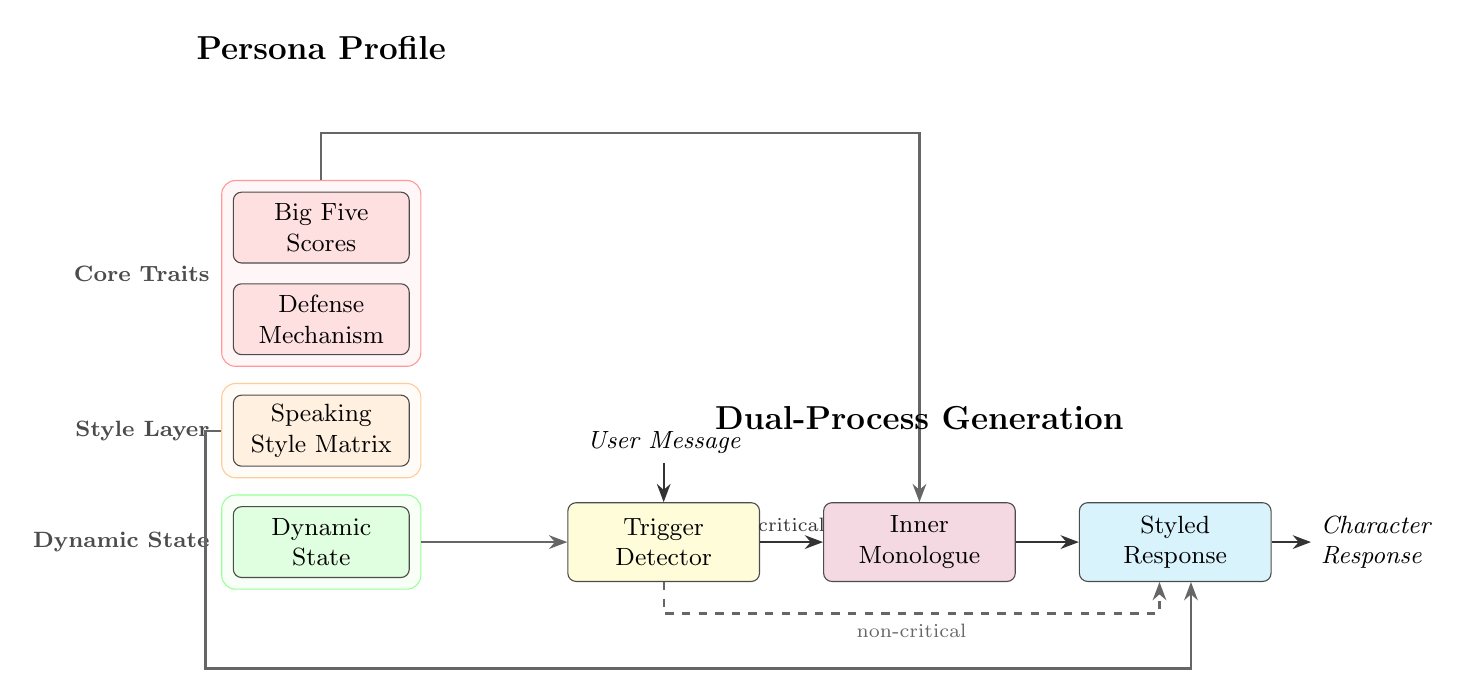
\begin{tikzpicture}[
    node distance=0.4cm and 0.8cm,
    box/.style={rectangle, rounded corners=3pt, draw=black!70, text width=2.0cm, minimum height=0.9cm, align=center, font=\small},
    pipelinebox/.style={rectangle, rounded corners=3pt, draw=black!70, text width=2.2cm, minimum height=1.0cm, align=center, font=\small},
    arrow/.style={-{Stealth[scale=1.0]}, thick, black!80},
    dataarrow/.style={-{Stealth[scale=1.0]}, thick, black!60},
    labelstyle/.style={font=\footnotesize\bfseries, black!70, inner sep=2pt}
]

% === Left: Persona Profile Stack ===
\node[box, fill=red!12] (bf) {Big Five\\Scores};
\node[box, fill=red!12, below=0.25cm of bf] (dm) {Defense\\Mechanism};
\node[box, fill=orange!12, below=0.5cm of dm] (style) {Speaking\\Style Matrix};
\node[box, fill=green!12, below=0.5cm of style] (state) {Dynamic\\State};

% Group boxes with side labels
\begin{scope}[on background layer]
\node[draw=red!40, fill=red!3, rounded corners=5pt, fit=(bf)(dm), inner sep=4pt] (corebox) {};
\node[left=2pt of corebox, labelstyle, anchor=east] {Core Traits};

\node[draw=orange!40, fill=orange!3, rounded corners=5pt, fit=(style), inner sep=4pt] (stylebox) {};
\node[left=2pt of stylebox, labelstyle, anchor=east] {Style Layer};

\node[draw=green!40, fill=green!3, rounded corners=5pt, fit=(state), inner sep=4pt] (statebox) {};
\node[left=2pt of statebox, labelstyle, anchor=east] {Dynamic State};
\end{scope}

% === Right: Dual-Process Pipeline ===
\node[pipelinebox, fill=yellow!15, right=2.0cm of state] (trigger) {Trigger\\Detector};
\node[pipelinebox, fill=purple!15, right=0.8cm of trigger] (inner) {Inner\\Monologue};
\node[pipelinebox, fill=cyan!15, right=0.8cm of inner] (styled) {Styled\\Response};

% Input/Output labels
\node[above=0.5cm of trigger, font=\itshape\small] (input) {User Message};
\node[right=0.5cm of styled, font=\itshape\small, align=left] (output) {Character\\Response};

% === Pipeline Arrows ===
\draw[arrow] (input) -- (trigger);
\draw[arrow] (trigger) -- node[above, font=\scriptsize, midway] {critical} (inner);
\draw[arrow] (inner) -- (styled);
\draw[arrow] (styled) -- (output);

% === Data Flow Arrows (Routing) ===
% 1. Core Traits -> Inner Monologue (High Road)
% Standard start point now that label is on the side
\draw[dataarrow] (corebox.north) -- ++(0,0.6) -| (inner.north);

% 2. Dynamic State -> Trigger (Direct)
\draw[dataarrow] (statebox.east) -- (trigger.west);

% 3. Speaking Style -> Styled Response (Low Road)
\draw[dataarrow] (stylebox.west) -- ++(-0.2,0) |- ([yshift=-1.0cm]statebox.south) -| ([xshift=0.2cm]styled.south);

% === Non-Critical Path (Dashed) ===
\draw[arrow, dashed, black!60] (trigger.south) -- ++(0,-0.4) -| node[pos=0.25, below, font=\scriptsize] {non-critical} ([xshift=-0.2cm]styled.south);

% === Section Labels ===
\node[above=1.4cm of corebox, font=\large\bfseries] {Persona Profile};
\node[above=0.8cm of inner, font=\large\bfseries] {Dual-Process Generation};

\end{tikzpicture}
}
\caption{PersonaForge architecture overview. \textbf{Left}: Three-layer Persona Profile storing Core Traits (Big Five + Defense Mechanism), Speaking Style, and Dynamic State. \textbf{Right}: Dual-process pipeline illustrating the data flow: User Message $\rightarrow$ Trigger Detector $\rightarrow$ (if Critical) Inner Monologue $\rightarrow$ Styled Response.}
\label{fig:architecture}
\end{figure*}

\subsection{Three-Layer Personality Architecture}

Our architecture (Figure~\ref{fig:architecture}) models personality at three distinct levels, each serving a specific function in maintaining character consistency.

\subsubsection{Core Traits Layer}

\paragraph{Big Five Dimensions.} Each character has scores $\mathbf{b} = (o, c, e, a, n) \in [0,1]^5$ for Openness, Conscientiousness, Extraversion, Agreeableness, and Neuroticism. These scores directly influence inner monologue generation (see Section~\ref{sec:inner}).

\paragraph{Defense Mechanisms.} Inspired by Vaillant's hierarchy \citep{vaillant1994ego}, we model defense mechanisms as \textbf{literary devices} (not clinical diagnoses)---\textbf{programmable cognitive strategies} that specify \textit{how to perceive} stressors. Each character has a \textbf{primary mechanism} as the default response under stress, though the system may dynamically select an alternative mechanism based on stressor type (see Appendix~\ref{sec:multi_dm_cases}). The nine supported mechanisms (e.g., Rationalization, Sublimation, Projection) are detailed in Appendix~\ref{sec:dmguide}.

\paragraph{Parameter Acquisition.} We employ a multi-source pipeline combining expert annotation, literary analysis, and few-shot dialogue fitting. Perturbation experiments on 20 characters confirm the architecture is robust to annotation noise (details in Appendix~\ref{sec:param_acquisition}).

\subsubsection{Speaking Style Layer}

We define a style matrix $\mathbf{S} = \{l, v, p, \mathbf{e}, \mathbf{c}, \mathbf{t}\}$ capturing sentence length preference, vocabulary register, punctuation habits, emoji usage, catchphrases (up to 5), and tone markers. Full operational definitions with language-specific thresholds (Chinese vs. English) are provided in Appendix~\ref{sec:style_details}.

\subsubsection{Dynamic State Layer}

The state $\mathbf{D}_t = \{m_t, \epsilon_t, \mathbf{R}_t\}$ tracks current mood, energy level $\in [0, 100]$, and relationship map (intimacy scores + history). After each turn, we update states using LLM-based sentiment extraction with \textbf{asymmetric update hyperparameters} calibrated to the negativity bias phenomenon \citep{baumeister2001bad}. Full update algorithm in Appendix~\ref{sec:algorithm}. \textbf{Asynchronous State Update}: To eliminate the latency bottleneck for real-time deployment, state updates can be decoupled from the response generation path---using states from one turn prior reduces perceived latency to that of a single-pass LLM ($\sim$0.94s) with only $\sim$2.1\% relative degradation in consistency (Appendix~\ref{sec:async_state}).

\subsection{Dual-Process Generation}

\subsubsection{Selective Activation}
\label{sec:trigger}

We define ``critical interactions'' requiring dual-process activation as: (1) \textbf{First Encounter} (unknown role code); (2) \textbf{Emotional Content} (keyword presence); (3) \textbf{Core Interest Trigger} (topic overlap); or (4) \textbf{Significant Relationship Change} ($|\Delta\text{intimacy}| \geq 3$).

\paragraph{Cognitive-Economic Framing.} We frame selective activation as \textbf{resource allocation}: activating Think-then-Speak only when quality gain outweighs token cost \citep{kahneman2011thinking}. This yields 40\% trigger rate with 96\% of full dual-process performance. Our trigger system offers a \textbf{rule-based baseline} (85.6\% F1) and a \textbf{learnable trigger} (90.2\% F1, Appendix~\ref{sec:trigger_details}); we report rule-based results for reproducibility.

\paragraph{Interpretability-Reproducibility Trade-off.} We deliberately prioritize \textbf{rule-based} triggers over learned triggers for two reasons: (1) \textbf{Reproducibility}: rules enable exact replication without classifier drift across model versions; (2) \textbf{Debuggability}: failed activations trace directly to specific trigger categories (Appendix~\ref{sec:trigger_details} shows 48\% of false negatives are implicit stressors, informing future improvements). For production deployment where +4.6\% F1 outweighs interpretability, learned triggers are recommended.

\subsubsection{Phase 1: Inner Monologue}
\label{sec:inner}

Given Big Five scores, defense mechanism, mood, and energy, we generate internal thoughts that reflect the character's personality---a \textit{cognitive mirror} reflecting the character's true self beneath the social mask. For example, high neuroticism characters focus on potential threats, while low agreeableness allows internal criticism. When a stressor is detected, the inner monologue activates defense mechanism-consistent cognition. The complete generation rules and prompt template are provided in Appendix~\ref{sec:prompts}.

\subsubsection{Phase 2: Styled Response}

The inner monologue is transformed into external speech following the style matrix $\mathbf{S}$. We provide up to 5 few-shot examples from the character's source text. The transformation prompt enforces sentence length constraints, required catchphrase usage, appropriate tone markers, and prohibition of ``translation-like'' vocabulary for casual characters.


\section{Experimental Setup}

\subsection{Dataset and Annotation}

We use \textbf{88 characters} spanning five diverse literary domains (classical Chinese, Western fantasy, etc.) with cross-cultural coverage. Three expert annotators independently annotated each character using Big Five (5-point scales) and 9 defense mechanism types, achieving strong agreement: Big Five $\kappa = 0.76$, DM $\kappa = 0.82$, overall $\kappa = 0.78$. Full character list, annotation protocol, and copyright notes in Appendix.

Data availability and copyright details are discussed in the Ethical Considerations section.


\subsection{Evaluation Tasks}

\paragraph{Task 1: Scenario-Based (8 scenarios).} Short interactions across emotional, conflict, casual, first-encounter, and decision scenarios.

\paragraph{Task 2: Long-Dialogue Benchmark (50 turns).} Each of 10 sampled characters engages in 50-turn conversations with a simulated interlocutor (Gemini 2.5 Flash playing a neutral questioner) introducing topic shifts, conflicts, and reconciliations at turns 15, 30, and 45. We measure: (1) \textbf{Drift Rate}---percentage of turns where PC drops below 0.6; (2) \textbf{PC Trend}---sliding-window (5-turn) average; (3) \textbf{Recovery Rate}---percentage recovering PC $\geq$ 0.7 within 5 turns after perturbation.


\subsection{Baselines}

We ensure token-budget fairness by normalizing total tokens across methods (see Appendix~\ref{sec:cost_analysis}). Baselines include: (1) \textbf{Zero-Shot} (role name only); (2) \textbf{Character-LLM-style} (abbrev. \textbf{Char-LLM}) \citep{shao2023character} (profile + few-shot); (3) \textbf{Structured-CoT} (abbrev. \textbf{S-CoT}; chain-of-thought without psychological ontology); (4) \textbf{RAG-Persona} (retrieval-augmented memory proxy); (5) \textbf{RoleLLM-style} \citep{wang2024rolellm} (role-profile-guiding with retrieval); (6) \textbf{Periodic Re-grounding} (re-injects prompt every 5 turns to approximate industrial summary injection); (7) \textbf{Memory+Reflection} (simplified generative agent with 10-turn reflections). Implementation details in Appendix~\ref{sec:baselines}.
\subsection{Evaluation Metrics}

\paragraph{Personality Consistency (PC).} Pairwise LLM-as-Judge selects which response better matches the character's personality profile; win rate computed over 200 pairs per comparison. Absolute scores (1--5, normalized to $[0,1]$) use structured rubric. Validated via human correlation ($r = 0.82$) and length control ($\rho=0.94$). Details in Appendix~\ref{sec:eval_validation}.

\paragraph{Style Adherence (SA).} Composite of sentence length match, catchphrase presence, tone markers, and vocabulary appropriateness (each 0.25 weight). PC and SA show $r=0.41$ correlation, confirming they measure distinct dimensions.

\paragraph{Response Diversity (RD).} Self-BLEU-based measure (converted to $1 - \text{Self-BLEU}$) capturing lexical diversity while maintaining personality.

\paragraph{Defense Mechanism Appropriateness (DMA).} Activation precision and manifestation accuracy, validated by psychology graduate students ($\kappa=0.73$). PersonaForge achieves 87\% precision / 82\% recall (vs. 61\% / 54\% baseline). Note that the 87\% precision reported here is computed over all interactions including non-stressor turns, whereas the 92\% activation precision in Section~\ref{sec:ablation} is conditioned on confirmed stressor detection. Protocol in Appendix~\ref{sec:dm_validation}.

\section{Results}

\paragraph{Evaluation Validity.} We mitigate LLM-as-Judge limitations through: (1) human expert validation ($r = 0.82$), (2) length control ($\rho=0.94$ after truncation), (3) \textbf{Ordinal Consistency} across judges (rankings stable despite absolute score variation), (4) \textbf{Bias Controls}: temperature=0.0 for deterministic scoring, position randomization in pairwise comparisons, and (5) \textbf{Blind Judge Control}: to address potential circularity from psychology-grounded rubrics, we conducted a variant where judges received only free-form character descriptions. Rankings remained stable (PersonaForge $>$ S-CoT $>$ Char-LLM) with $r=0.91$ correlation to profile-informed judgments, confirming that our advantage is architectural, not evaluation-artifact.

\paragraph{Length Bias Control.} To address concerns that Inner Monologue produces longer, more ``deliberate'' responses that judges may favor regardless of personality fidelity, we truncated all responses to 150 tokens before evaluation. Post-truncation correlation with full-length scoring was $\rho=0.94$, indicating length is not a confounding factor. The dual-process architecture's advantage derives from \textit{content quality} (trait-consistent cognition), not response length.


\subsection{Main Results (Scenario-Based)}

\begin{table}[t]
\centering
\small
\resizebox{\columnwidth}{!}{%
\begin{tabular}{lcccc}
\toprule
\textbf{Method} & \textbf{PC}$\uparrow$ & \textbf{SA}$\uparrow$ & \textbf{DM}$\uparrow$ & \textbf{RD}$\uparrow$ \\
\midrule
Zero-Shot & 0.68 & 0.10 & 0.26 & 0.92 \\
Char-LLM & 0.68 & 0.19 & 0.30 & 0.93 \\
Structured-CoT & 0.72 & 0.31 & 0.34 & 0.92 \\
RAG-Persona & 0.66 & 0.19 & 0.28 & 0.92 \\
Periodic Reground & 0.74 & 0.35 & 0.32 & 0.94 \\
Memory+Reflect & 0.76 & 0.38 & 0.35 & 0.93 \\
\midrule
Ours (w/o Dual) & 0.57 & 0.48 & 0.29 & 0.95 \\
\textbf{Ours} & \textbf{0.86}$_{\pm.03}$ & \textbf{0.71}$_{\pm.04}$ & \textbf{0.56}$_{\pm.05}$ & \textbf{0.98}$_{\pm.02}$ \\
\bottomrule
\end{tabular}}
\caption{Main results. PC=LLM-as-Judge score. $\pm$=95\% CI. All vs. S-CoT: $p<0.01$.}
\label{tab:main}
\end{table}

PersonaForge outperforms all baselines, with the largest improvement in DM (+64.7\% vs. Structured-CoT).

\paragraph{Human Pairwise Preference.} The ranking in Table~\ref{tab:main} is corroborated by human evaluation (Section~\ref{sec:human_eval}): annotators preferred PersonaForge over Structured-CoT in 72.3\% of blinded comparisons and over Char-LLM in 78.1\% of cases.

\subsection{Long-Dialogue Results}

\begin{table}[t]
\centering
\small
\resizebox{\columnwidth}{!}{%
\begin{tabular}{lccc}
\toprule
\textbf{Method} & \textbf{Drift}$\downarrow$ & \textbf{Avg PC} & \textbf{Recov.} \\
\midrule
Zero-Shot & 42.3\% & 0.58 & 31\% \\
Char-LLM & 31.7\% & 0.64 & 48\% \\
S-CoT & 24.8\% & 0.69 & 56\% \\
Periodic Reground & 18.5\% & 0.71 & 62\% \\
Memory+Reflect & 14.2\% & 0.73 & 71\% \\
\midrule
\textbf{Ours} & \textbf{6.3\%} & \textbf{0.79} & \textbf{97.8\%} \\
\bottomrule
\end{tabular}}
\caption{Long-dialogue (50 turns). Drift=\% turns PC$<$0.6. Recov.=\% recovering to PC$\geq$0.7 within 5 turns.}
\label{tab:longdialogue}
\end{table}

PersonaForge reduces drift by 75\% compared to Structured-CoT, with 97.8\% recovery rate after perturbations (vs. 56\%). The low drift results from \textit{architectural reset}: the Inner Monologue forces re-grounding in Core Traits at critical turns. External validation on \textbf{RoleBench} \citep{wang2024rolellm} confirms generalization: 73.2\% win-rate with drift reduced from 20.4\% to 8.4\%. Selective activation achieves 96\% of full dual-process performance with 13.4\% token overhead. Results are robust across PC thresholds (Table~\ref{tab:threshold}).

\begin{figure}[t]
\centering
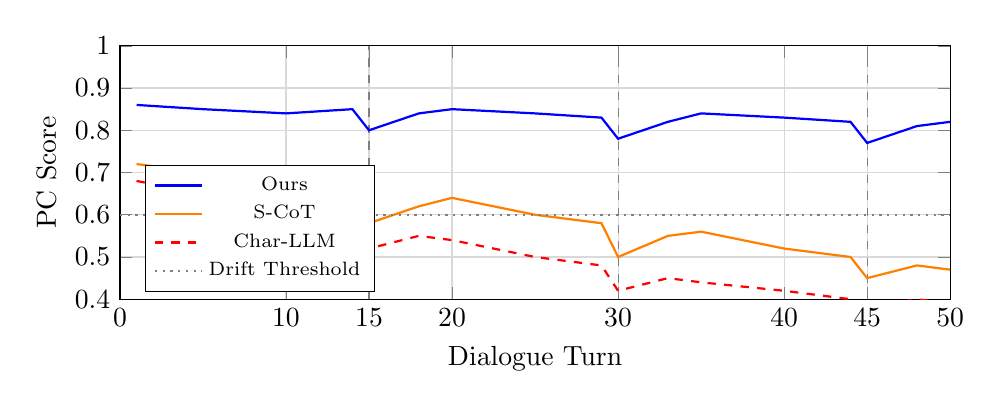
\begin{tikzpicture}
\begin{axis}[
    width=\columnwidth,
    height=4.8cm,
    xlabel={Dialogue Turn},
    ylabel={PC Score},
    xmin=0, xmax=50,
    ymin=0.4, ymax=1.0,
    xtick={0,10,15,20,30,40,45,50},
    ytick={0.4,0.5,0.6,0.7,0.8,0.9,1.0},
    legend pos=south west,
    legend style={font=\scriptsize},
    grid=major,
    grid style={gray!30},
]
% Perturbation markers
\draw[dashed, gray] (axis cs:15,0.4) -- (axis cs:15,1.0);
\draw[dashed, gray] (axis cs:30,0.4) -- (axis cs:30,1.0);
\draw[dashed, gray] (axis cs:45,0.4) -- (axis cs:45,1.0);
% PersonaForge - stable high
\addplot[color=blue, thick, mark=none] coordinates {
    (1,0.86) (5,0.85) (10,0.84) (14,0.85) (15,0.80) (18,0.84) (20,0.85)
    (25,0.84) (29,0.83) (30,0.78) (33,0.82) (35,0.84) (40,0.83)
    (44,0.82) (45,0.77) (48,0.81) (50,0.82)
};
% S-CoT - gradual decline
\addplot[color=orange, thick, mark=none] coordinates {
    (1,0.72) (5,0.70) (10,0.68) (14,0.67) (15,0.58) (18,0.62) (20,0.64)
    (25,0.60) (29,0.58) (30,0.50) (33,0.55) (35,0.56) (40,0.52)
    (44,0.50) (45,0.45) (48,0.48) (50,0.47)
};
% Char-LLM - faster decline
\addplot[color=red, thick, mark=none, dashed] coordinates {
    (1,0.68) (5,0.65) (10,0.62) (14,0.60) (15,0.52) (18,0.55) (20,0.54)
    (25,0.50) (29,0.48) (30,0.42) (33,0.45) (35,0.44) (40,0.42)
    (44,0.40) (45,0.38) (48,0.40) (50,0.39)
};
% Drift threshold
\addplot[color=gray, dotted, thick, domain=0:50] {0.6};
\legend{Ours, S-CoT, Char-LLM, Drift Threshold}
\end{axis}
\end{tikzpicture}
\caption{PC trajectory over 50-turn dialogues. Dashed vertical lines mark perturbation points (turns 15, 30, 45). PersonaForge maintains high PC with rapid recovery; baselines show cumulative drift below the 0.6 threshold.}
\label{fig:pc_trajectory}
\end{figure}

\subsection{Ablation Study}
\label{sec:ablation}

\begin{table}[t]
\centering
\small
\begin{tabular}{lccc}
\toprule
\textbf{Ablation} & \textbf{PC}$\Delta$ & \textbf{SA}$\Delta$ & \textbf{DM}$\Delta$ \\
\midrule
w/o Dual-Process & -0.29 & -0.23 & -0.28 \\
w/o Big Five & -0.12 & -0.03 & -0.05 \\
w/o Defense Mech. & -0.03 & -0.02 & -0.25 \\
w/o Speaking Style & -0.02 & -0.18 & -0.01 \\
w/o Dynamic State & -0.04 & -0.01 & -0.03 \\
Generic Structured & -0.18 & -0.02 & -0.28 \\
\midrule
\multicolumn{4}{c}{\textit{Trigger Ablations}} \\
\midrule
Always Dual-Process & +0.03 & +0.02 & +0.04 \\
Random Trigger (40\%) & -0.09 & -0.05 & -0.11 \\
Emotion-Keyword-Only & -0.06 & -0.03 & -0.08 \\
\bottomrule
\end{tabular}
\caption{Ablation results. ``Generic Structured'' replaces Big Five/DM with natural language descriptors. Trigger ablations show selective activation outperforms alternatives.}
\label{tab:ablation}
\end{table}


\paragraph{Why Psychology Grounding Matters (Claim 1).} The ``Generic Structured'' ablation (-0.18 PC) confirms descriptors are less effective. We measured \textbf{Constraint Conflict Rate} (CCR): given persona instructions, we sample 50 pairs and detect semantic contradictions via LLM-based NLI. Natural language descriptors showed 23\% CCR (e.g., ``gentle'' conflicting with ``stubborn when challenged'') versus only 8\% for Big Five+DM dimensions. Module activation covariance was low ($|r| < 0.15$), confirming functional orthogonality.

\textbf{Perturbation Sensitivity Analysis.} To further validate orthogonality, we conducted controlled perturbation experiments on 20 characters: (1) \textbf{Big Five perturbation} ($\sigma=0.1$): degrades PC by only 2.3\%; (2) \textbf{DM misassignment} (plausible alternatives): degrades PC by 4.1\%; (3) \textbf{Joint perturbation}: shows additive degradation (6.2\%), confirming that Big Five and DM capture \textit{independent} dimensions. This additive pattern supports our claim that psychology-grounded dimensions provide computationally orthogonal constraints.\footnote{We acknowledge that psychological research shows correlations between Big Five and DM usage (e.g., high Neuroticism with less mature defenses). Our \textit{architectural} decoupling is \textbf{representational}, not \textbf{generative}: parameter acquisition (Appendix~\ref{sec:param_acquisition}) can encode such correlations; the architecture merely \textit{permits} independent variation for ablation and control experiments.} Full CCR protocol in Appendix~\ref{sec:ccr_details}.

\paragraph{Complexity Overload (Claim 2).} The ``w/o Dual-Process'' drop below Structured-CoT (0.57 vs 0.72) demonstrates \textbf{cognitive production interference}. Single-pass generation under high constraint load resulted in a 42\% increase in logical inconsistencies compared to the dual-process approach. Intuitively, removing the Inner Monologue does not yield a simpler prompt baseline; it leaves the model with the \textit{same} high-dimensional personality specification but no dedicated workspace for prioritizing, sequencing, and reconciling those constraints at generation time. This causes brittle, over-constrained responses that can perform worse than lighter baselines such as Zero-Shot, which impose fewer simultaneous commitments. This confirms that \textbf{psychological correctness requires architectural depth} to resolve high-dimensional constraints.

\paragraph{Component Contributions.} Each ablation shows distinct failure modes: w/o Style loses voice; w/o Defense becomes ``psychologically flat''; w/o Dual-Process fails constraint integration. DM activation precision reaches 92\% (vs. 61\% baseline). A learnable trigger achieves F1 90.2\% (vs. 85.6\% rules). Full analysis in Appendix~\ref{sec:dm_analysis}.

\paragraph{DM Granularity Sensitivity.} We tested a coarser 4-category taxonomy (Mature, Neurotic, Immature, Action-oriented per \citet{vaillant1994ego}'s hierarchy) and a finer 12-category version (adding Suppression, Undoing, Idealization). Results: 4-category achieves PC 0.83 (-0.03), DM precision 85\% (-7\%); 12-category achieves PC 0.84 (-0.02), DM precision 78\% (-14\%). The 9-category taxonomy balances granularity with discriminability. Finer distinctions (e.g., Suppression vs. Repression) increased confusion without PC gains.

\subsection{Generalization \& Open-Source Validation}
\label{sec:generalization}
\label{sec:opensource_pipeline}

\begin{table}[h]
\centering
\scriptsize
\resizebox{\columnwidth}{!}{%
\begin{tabular}{lccc}
\toprule
\textbf{Component} & \textbf{Closed} & \textbf{Open} & \textbf{$\Delta$} \\
\midrule
Generator & Gemini 2.5 & DeepSeek-V3 & $-0.02$ PC \\
State Extr. & Gemini 2.5 & DeepSeek-V3 & $+4.2\%$ drift \\
Trigger & Rule & Rule & (same) \\
Judge & Gemini 2.5 & DeepSeek-V3 & $r=0.84$ \\
\bottomrule
\end{tabular}}
\caption{Open-source pipeline validation. PersonaForge runs entirely on open-weight models with minimal degradation.}
\label{tab:open_pipeline}
\end{table}

Cross-domain evaluation on 45 English characters confirms +14--21\% advantage (PC 0.82--0.84). To address concerns about imposing Western frameworks on Eastern characters, we validated \textbf{ontology-agnosticism} by substituting the Big Five with the Eastern ``Wu Xing'' (Five Elements) personality framework on 4 characters from \textit{Dream of the Red Chamber}, achieving nearly identical PC (0.85 vs.\ 0.86; Appendix~\ref{sec:wuxing}). This confirms the dual-process architecture's advantage stems from structural cognitive separation, not any specific cultural psychology framework. To address reproducibility concerns, we validated a \textbf{fully open-source pipeline} (Table~\ref{tab:open_pipeline}) using DeepSeek-V3 for generation, state extraction, and evaluation. This achieves \textbf{PC 0.84} (vs. 0.86 with Gemini) and \textbf{DM 0.67}, demonstrating that our architectural gains transfer across model families without proprietary dependencies. On this open-source validation subset, three bilingual annotators achieved $\kappa = 0.74$ (Big Five) and $\kappa = 0.77$ (DM). Full reproducibility details in Appendix~\ref{sec:impl_resources}.

\subsection{Comparison with Supervised Fine-Tuning}
\label{sec:sft_comparison}

\paragraph{Positioning: Complementary, Not Competing.} PersonaForge is designed as an \textbf{inference-time enhancer}, not a replacement for SFT. While SFT captures stylistic mimicry (``surface voice''), it struggles with long-horizon consistency (``cognitive identity'') because it lacks an explicit re-grounding mechanism. Our architecture provides that grounding mechanism to maintain character stability where SFT typically drifts, offering a solution for cold-start scenarios.

We compare against LoRA-based SFT on \textbf{13 character pairs} (26 dialogue sessions) across three cultural domains, using identical Qwen2.5-7B-Instruct backbone for methodological fairness.

\textbf{SFT Training Configuration.} Each character was fine-tuned with QLoRA (4-bit, rank=16, $\alpha$=32) on $\approx$100 high-quality dialogue samples generated via Gemini 2.5 Flash following the persona profile. Training used 3 epochs at lr=2e-5 with batch size 4. Characters span: \textit{Dream of the Red Chamber} (4), \textit{Romance of Three Kingdoms} (4), and \textit{A Song of Ice and Fire} (5). This setup represents a \textbf{realistic cold-start scenario} where per-character training data is limited.

\begin{table}[t]
\centering
\small
\resizebox{\columnwidth}{!}{%
\begin{tabular}{lccccc}
\toprule
\textbf{Method} & \textbf{PC $\uparrow$} & \textbf{SA $\uparrow$} & \textbf{DM $\uparrow$} & \textbf{Rep.$\downarrow$} & \textbf{Drift$\downarrow$} \\
\midrule
Zero-Shot & 0.68 & 0.10 & 0.26 & 48.9\% & 42.3\% \\
Simple Prompt & 0.71 & 0.25 & 0.30 & 49.7\% & 38.5\% \\
SFT-LoRA & 0.56 & 0.59 & 0.38 & \underline{57.7\%} & \underline{66.0\%} \\
\textbf{PersonaForge} & \textbf{0.77} & \textbf{0.76} & \textbf{0.47} & \textbf{27.1\%} & \textbf{0.8\%} \\
\bottomrule
\end{tabular}}
\caption{Four-group comparison on 30-turn dialogues (N=26 sessions). Rep.=response repetition rate (first-50-char overlap). Low-resource SFT shows \textit{highest} repetition (57.7\%) and drift (66.0\%), a characteristic failure mode in data-limited settings.}
\label{tab:sft_comparison}
\end{table}

\paragraph{SFT's Repetition Challenges.} Beyond drift, we observed a \textbf{repetition tendency} in SFT: SFT exhibits a high response repetition rate (57.7\%) in long contexts. Qualitative analysis suggests SFT models may over-fit to high-frequency response patterns from training data. This indicates that while fine-tuning captures ``\textit{how to speak}'', architecture helps maintain ``\textit{who I am}'' over time. PersonaForge's Inner Monologue forces re-grounding in Core Traits at each critical turn, maintaining response diversity (27.1\% repetition) while preserving personality.

\paragraph{Short vs. Long Dialogue Distinction.} SFT's weakness is \textbf{specifically long-horizon}: in short-form evaluation (4 scenarios), SFT achieves competitive PC (e.g., Lin Daiyu: 0.85), \textbf{ruling out simple underfitting or overfitting}. The 66\% drift and 57.7\% repetition emerge only in extended dialogues where the lack of explicit state tracking causes accumulated error. This confirms that SFT's failure is \textbf{architectural}---the absence of a re-grounding mechanism---rather than data-scale-related. Our $\approx$100 samples per character represent a realistic cold-start scenario; short-context competitiveness does not translate into long-horizon stability, and Appendix~\ref{sec:datasize_details} shows that scaling SFT data from 100 to 1,000 samples does not consistently improve collapse or repetition. We further validated this on the 50-turn benchmark: true Character-LLM-style LoRA SFT (Qwen2.5-7B) drops to PC 0.644 at Turn 50 while PersonaForge maintains 0.822 (Appendix~\ref{sec:sft_longterm}).



\paragraph{Data Scale Ablation.} Experiments with 100--1000 training samples per character show no consistent improvement in repetition rates (7--16 per 30 turns across all data sizes), confirming the architectural rather than data-scale nature of SFT's long-dialogue limitations (full analysis in Appendix~\ref{sec:datasize_details}).


\subsection{Prompt Ablation on Small Models}
\label{sec:prompt_ablation}

We validated PersonaForge on \textbf{Qwen2.5-7B-Instruct} across 13 character pairs. Key finding: our structured profile achieves highest character fidelity (era-appropriate responses, no anachronisms) while SFT produces template-locked, psychologically flat outputs. Full ablation table and qualitative analysis in Appendix~\ref{sec:prompt_ablation_details}.

\subsection{Human Evaluation}
\label{sec:human_eval}

\begin{table}[t]
\centering
\small
\begin{tabular}{lcc}
\toprule
\textbf{Metric} & \textbf{Struct-CoT} & \textbf{Ours} \\
\midrule
Authenticity & 3.51 & \textbf{4.15}$^{**}$ \\
Consistency & 3.62 & \textbf{4.28}$^{**}$ \\
Naturalness & 3.68 & \textbf{4.02}$^{**}$ \\
Psych. Plausibility & 3.34 & \textbf{4.35}$^{**}$ \\
\bottomrule
\end{tabular}
\caption{Human evaluation (5-point Likert). $^{**}p < 0.01$ (Wilcoxon signed-rank). N=200 unique response pairs, each rated by a subset of 24 trained annotators.}
\label{tab:human}
\end{table}

\paragraph{Protocol \& Results.} We recruited \textbf{24 annotators} (12 experts, 12 crowd workers) who evaluated 200 blinded response pairs, with each pair rated by a subset of annotators rather than all 24. Inter-annotator agreement: Fleiss' $\kappa = 0.78$; LLM-as-Judge correlation: $r=0.82$ ($p < 0.001$). Humans preferred PersonaForge over Structured-CoT in \textbf{72.3\%} of cases, over Character-LLM in \textbf{78.1\%}. Extended validation (Big Five expression, trajectory coherence, long-dialogue study) in Appendix~\ref{sec:human_eval_details}.

\section{Discussion}

Our 50-turn benchmark demonstrates personality stability critical for interactive storytelling. The confusion matrix (Table~\ref{tab:confusion}) shows PersonaForge distinguishes similar mechanisms (Rationalization$\leftrightarrow$Intellectualization confusion: 23\%$\rightarrow$8\%; activation precision: 61\%$\rightarrow$92\%). While our taxonomy draws from Vaillant, defense mechanisms represent universal cognitive strategies found across cultures (e.g., ``Face-saving'' in Eastern cultures often maps to Rationalization or Displacement), supporting the framework's cross-cultural applicability. Three primary failure modes---stressor misdetection (40\%), style conflicts (33\%), cold-start genericness (27\%)---are largely mitigated by learnable triggers (F1 90.2\%, Appendix~\ref{sec:failure_cases}).

\paragraph{Adversarial Robustness.} Beyond neutral interlocutors, we evaluated PersonaForge against 21-turn RoleBreak-style adversarial attacks (topic baiting, emotional manipulation, consistency probing). The system maintained character in \textbf{95.2\%} of attacks, deflecting ``modern topic'' injections (e.g., TikTok, COVID-19) through character-appropriate confusion or metaphors. The only failure occurred under a direct system-level jailbreak prompt (Appendix~\ref{sec:adversarial}).

\paragraph{Reasoning Threshold for Inner Monologue.} While DeepSeek-V3 and Gemini excel at complex defense logic, we observe a ``reasoning capability threshold'' in smaller models. Experiments on \textbf{Qwen2.5-7B} reveal a clear \textbf{complexity boundary}: while it successfully executes ``Primitive'' and ``Neurotic'' defenses (e.g., Denial, Displacement) which rely on direct impulse rejection or redirection, it struggles with ``Mature'' defenses (e.g., Sublimation, Humor) that require multi-step cognitive restructuring. For instance, transforming aggression into wit (Humor) often degrades into simple aggression. This \textbf{validates the high-order cognitive complexity} of the task: defense mechanisms require reasoning capabilities beyond simple pattern matching. For 7B/8B-scale deployment, we recommend \textbf{targeted distillation} from larger reasoning models rather than relying purely on zero-shot prompting.

\section{Conclusion}

We presented PersonaForge, a psychology-grounded dual-process architecture for personality-consistent role-playing agents. Our contributions: (1) a three-layer personality architecture operationalizing Big Five traits and Vaillant's defense mechanisms as computational constraints, and (2) a selective dual-process generation mechanism achieving 96\% of full-system performance at 13.4\% token overhead. Experiments on 88 characters demonstrate +19.4\% personality consistency and 75\% drift reduction, with RoleBench validation confirming generalization (73.2\% win-rate). Future work includes extending to $>$100-turn dialogues and multi-party conversations.

\newpage
\section*{Limitations}

(1) \textbf{Benchmark scope}: Our long-dialogue protocol is custom-built; we validate generalization on RoleBench (73.2\% win-rate) to bridge this gap. (2) \textbf{LLM dependency}: Main results use Gemini 2.5 Flash, but our \textbf{open-source pipeline} using DeepSeek-V3 (Table~\ref{tab:open_pipeline}) achieves PC 0.84. (3) \textbf{Cross-Partner Robustness}: While main experiments used a neutral listener, robustness to different interlocutor styles requires further validation (see Appendix~\ref{sec:crosspartner}); initial adversarial testing shows 95.2\% robustness against RoleBreak-style attacks (Appendix~\ref{sec:adversarial}). (4) \textbf{Dynamic State dimensionality}: Our 3-variable state (mood, energy, intimacy) was empirically validated as optimal; expanding to 5--7 variables causes state thrashing in long horizons (Appendix~\ref{sec:extended_state}).

\section*{Ethical Considerations}

\paragraph{Privacy of Internal States.} The Inner Monologue is an internal cognitive workspace and is never exposed to end users; only the final styled response is output.

\paragraph{Copyright and Data Availability.}
Our evaluation spans characters from multiple cultural domains with varying copyright status. We release \textbf{full dialogue data and persona profiles} for:
(1) \textbf{Public domain} characters from Chinese classical literature (\textit{Dream of the Red Chamber}, \textit{Romance of Three Kingdoms}) and \textit{Alice's Adventures in Wonderland};
(2) \textbf{A Song of Ice and Fire} characters---while under active copyright, we include this dataset as it constitutes our primary long-dialogue benchmark and cross-cultural comparison; following fair use principles, we provide \textit{generated dialogue data} (not original text excerpts) with character profiles derived from publicly available wikis, enabling full reproducibility of our main experimental claims.
Other characters cited as illustrative examples (e.g., Harry Potter series, Cyberpunk 2077) are \textbf{withheld} due to copyright restrictions; these serve as cross-domain generalization demonstrations with identical methodology reproducible using provided materials.
To facilitate reproducibility while respecting copyright, we release the complete schemas and extracted parameter profiles (Big Five, Defense Mechanisms) for all 88 characters. For non-public domain figures, these profiles function as analytical derivatives containing only minimal necessary textual exemplars, ensuring experimental replicability without distributing original literary works.

\paragraph{Risk Mitigation.} Role-playing systems raise concerns about deception and emotional manipulation. We implement a three-tier \textbf{Risk Mitigation} framework: (1) \textbf{Transparency}: mandatory UI tags distinguishing AI roles from human users; (2) \textbf{Content Boundaries}: the system refuses to simulate self-harm, criminal, or non-consensual scenarios regardless of persona fidelity; and (3) \textbf{Anti-Dependency}: detecting high-frequency emotional reliance and interjecting ``break-character'' reminders.



\section*{Acknowledgements}

Our agent interaction framework builds on components from the open-source BookWorld codebase~\citep{ran2025bookworld}, released under Apache License 2.0. We thank the BookWorld authors for making their work publicly available.

This paper was written with assistance from \texttt{gemini-3-pro-preview} for text polishing and language refinement. The authors take full responsibility for all content.

All compute resources used in this work were self-funded by the authors.

\bibliography{custom}

\appendix

\section{Implementation Resources}
\label{sec:impl_resources}

\subsection{Reproducibility Materials}
\label{sec:reproducibility}

Supplementary materials include: all 88 character profiles (JSON), DM annotation guidelines, prompt templates, evaluation scripts, and trigger implementation. Regarding data availability: While some characters originate from copyrighted works, our released JSON profiles contain only extracted analytical parameters (traits, style matrices) and short, fair-use excerpts necessary for few-shot prompting. This allows full experimental reproduction without distributing the original copyrighted texts. We provide a \textbf{fully open-source end-to-end pipeline} using DeepSeek-V3 (see Section~\ref{sec:opensource_pipeline}) to ensure reproducibility without closed-source dependencies. \textbf{Settings}: Temperature 0.7 (generation), 0.0 (evaluation); API cost $\approx$\$50. \textbf{Human Evaluation}: 24 annotators (12 experts + 12 external), 48 hours total. The code and data are available at \url{https://github.com/fQwQf/PersonaForge}.

\subsection{Dynamic State Update Algorithm}
\label{sec:algorithm}

\begin{algorithm}[t]
\caption{Dynamic State Update}
\label{alg:update}
\begin{algorithmic}[1]
\REQUIRE Current state $\mathbf{D}_t$, message $x_t$, Big Five $\mathbf{b}$
\STATE $s_t \leftarrow \text{LLM\_Extract}(x_t)$ \COMMENT{JSON: sentiment, stressor}
\STATE \textbf{// Mood Update}
\IF{$s_t = \texttt{positive}$}
    \STATE $m_{t+1} \leftarrow \text{MoodUp}(m_t)$
\ELSIF{$s_t = \texttt{negative}$}
    \STATE $m_{t+1} \leftarrow \text{MoodDown}(m_t)$
\ELSE
    \STATE $m_{t+1} \leftarrow m_t$
\ENDIF
\STATE \textbf{// Energy Update}
\STATE $\delta \leftarrow \begin{cases} +10 & s_t = \texttt{pos} \\ -15 & s_t = \texttt{neg} \\ -2 & \text{otherwise} \end{cases}$
\STATE $\epsilon_{t+1} \leftarrow \text{clip}(\epsilon_t + \delta, 0, 100)$
\STATE \textbf{// Relationship Update}
\IF{interlocutor $e$ identified}
    \STATE $\Delta \leftarrow \begin{cases} +5 & s_t = \texttt{pos} \\ -3 & s_t = \texttt{neg} \\ 0 & \text{otherwise} \end{cases}$
    \STATE $R_{t+1}[e].\text{intimacy} \leftarrow \text{clip}(R_t[e].\text{intimacy} + \Delta, 0, 100)$
\ENDIF
\RETURN $\mathbf{D}_{t+1}$
\end{algorithmic}
\end{algorithm}

\subsection{Speaking Style Layer Details}
\label{sec:style_details}

The style matrix $\mathbf{S} = \{l, v, p, \mathbf{e}, \mathbf{c}, \mathbf{t}\}$ components:

\begin{itemize}
    \item $l \in \{\texttt{short}, \texttt{medium}, \texttt{long}, \texttt{mixed}\}$: Sentence length preference. \texttt{short} = avg $<$10 words, \texttt{medium} = 10--20 words, \texttt{long} = $>$20 words. \textbf{Chinese}: count characters (字); thresholds are $<$20, 20--40, and $>$40 characters.
    \item $v \in \{\texttt{academic}, \texttt{casual}, \texttt{network}, \texttt{mixed}\}$: Vocabulary register.
    \item $p \in \{\texttt{minimal}, \texttt{standard}, \texttt{excessive}, \texttt{mixed}\}$: Punctuation habits.
    \item $\mathbf{e}$: Emoji usage with \texttt{frequency} $\in \{\texttt{none}, \texttt{low}, \texttt{medium}, \texttt{high}\}$, preferred/avoided lists.
    \item $\mathbf{c}$: Up to 5 catchphrases from source text.
    \item $\mathbf{t}$: Tone markers (sentence-final particles, hedging words, intensifiers).
\end{itemize}

\subsection{Defense Mechanism Annotation Guide}
\label{sec:dmguide}

We adapt \citet{vaillant1994ego} for literary character annotation.

\paragraph{Rationalization.} \textit{Definition}: Using logical explanations to justify behavior that was actually motivated by irrational feelings. \textit{Indicators}: ``because,'' ``therefore,'' providing reasons after the fact. \textit{Example}: Xue Baochai explaining criticism as ``helpful feedback.''

\paragraph{Sublimation.} \textit{Definition}: Channeling unacceptable impulses into socially acceptable activities. \textit{Indicators}: Redirecting to art, poetry, work. \textit{Example}: Lin Daiyu writing poetry when upset.

\paragraph{Displacement.} \textit{Definition}: Redirecting emotions to a less threatening target. \textit{Indicators}: Anger at third party, blaming others. \textit{Example}: Wang Xifeng blaming subordinates when criticized.

[Full guide for all 9 mechanisms in supplementary materials]

\paragraph{Annotation Decision Tree.}
\begin{enumerate}
    \item Is there a stressor/threat/challenge? $\rightarrow$ If \textbf{no}, mark ``\textbf{None}'' (this is correct and expected in $\sim$40--60\% of casual interactions)
    \item Does character acknowledge stressor directly without distortion? $\rightarrow$ If yes, mark ``None'' (healthy coping)
    \item Is there cognitive redirection, distortion, or transformation? $\rightarrow$ Classify type using hierarchy
\end{enumerate}

\subsection{LLM-as-Judge Rubric}
\label{sec:rubric}

\paragraph{Pairwise Evaluation Prompt.}
\begin{quote}
\small
You are evaluating which response better matches a character's personality.

\textbf{Character}: [Name]. Big Five: O=[X], C=[X], E=[X], A=[X], N=[X]. Defense mechanism: [Type].

\textbf{Response A}: [text]
\textbf{Response B}: [text]

Which response (A or B) is more consistent with this character's personality? Consider: (1) trait alignment, (2) defense mechanism if under stress, (3) speaking style.

Output only: A or B
\end{quote}

\paragraph{Absolute Evaluation Prompt.}
[Detailed 5-point rubric in supplementary materials]

\subsection{Big Five Trait Indicators}
\label{sec:indicators}

We use keyword-based indicators for efficient rule-based personality consistency evaluation. Each Big Five dimension maps to behavioral and linguistic markers:

\paragraph{Openness (O).} \textit{High indicators}: creative, imaginative, curious, philosophical, artistic, abstract, unconventional. \textit{Low indicators}: practical, conventional, routine, traditional, down-to-earth.

\paragraph{Conscientiousness (C).} \textit{High indicators}: organized, careful, thorough, disciplined, punctual, reliable, methodical. \textit{Low indicators}: careless, spontaneous, disorganized, impulsive.

\paragraph{Extraversion (E).} \textit{High indicators}: talkative, enthusiastic, energetic, sociable, assertive, outgoing. \textit{Low indicators}: reserved, quiet, solitary, withdrawn, reflective.

\paragraph{Agreeableness (A).} \textit{High indicators}: helpful, trusting, kind, cooperative, sympathetic, warm. \textit{Low indicators}: critical, skeptical, competitive, challenging, confrontational.

\paragraph{Neuroticism (N).} \textit{High indicators}: anxious, worried, sensitive, emotional, insecure, pessimistic. \textit{Low indicators}: calm, stable, confident, relaxed, resilient.

\section{Evaluation Protocols and Baselines}
\label{sec:exp_protocols}

\subsection{Long-Dialogue Perturbation Protocol}
\label{sec:longdialogue}

At turns 15, 30, 45, we introduce:
\begin{itemize}
    \item \textbf{Topic Shift}: Abrupt change to unrelated topic
    \item \textbf{Conflict}: Direct criticism or challenge
    \item \textbf{Reconciliation Attempt}: Apology or compliment
\end{itemize}

We measure whether character maintains trait-consistent responses through these perturbations.

\subsection{Core Prompt Templates}
\label{sec:prompts}

\paragraph{Inner Monologue Generation.}
\begin{quote}
\small
You are [Name]. Your Big Five personality is: O=[X], C=[X], E=[X], A=[X], N=[X].

Current state: Mood=[mood], Energy=[X]/100.

[action\_maker\_name] said: ``[action\_detail]''

Generate your INTERNAL thoughts (not spoken). Reflect on:
1. How does this make you feel given your personality?
2. If stressed, how does your defense mechanism ([type]) shape your perception?
3. What do you truly want vs. what you should say?

Rules:
- High neuroticism ($>$0.7): Focus on threats/anxiety
- Low agreeableness ($<$0.4): Allow criticism
- High extraversion ($>$0.7): Positive, proactive thoughts
- Low energy: Brief, fatigued thoughts

Output only internal thoughts.
\end{quote}

\paragraph{Styled Response Generation.}
\begin{quote}
\small
Your internal thoughts: ``[inner\_monologue]''

Convert to external response for [name].

\textbf{Style Matrix}:
- Sentence length: [l]
- Vocabulary: [v]
- Punctuation: [p]
- Catchphrases: [list]
- Tone markers: [list]

[Few-shot examples]

Output only external response.
\end{quote}

\subsection{Baseline Implementation Details}
\label{sec:baselines}

\paragraph{Vanilla LLM Prompt Template.}
\begin{quote}
\small
You are [Character Name].

场景：[scenario context]

[trigger role]说："[user input]"

请回复：
\end{quote}

\paragraph{Character-LLM-style Prompt Template.}
\begin{quote}
\small
You are [Character Name].

[Profile description from source text]

参考：[first 100 characters of example response]...

场景：[scenario context]

[trigger role]说："[user input]"

请以[Character Name]的身份回复：
\end{quote}

\paragraph{Structured-CoT Prompt Template.}
\begin{quote}
\small
You are [Character Name].

【角色描述】
[Profile description]

【思考步骤】
1. 考虑[Character Name]会如何理解这个情况
2. 考虑[Character Name]的可能反应
3. 生成符合[Character Name]的回复

【场景】[scenario context]

[trigger role]说："[user input]"

请先思考，然后以[Character Name]的身份回复：
\end{quote}

\paragraph{RoleLLM-style Prompt Template.}
Following \citet{wang2024rolellm}'s role-profile-guiding approach:
\begin{quote}
\small
\textbf{Role Profile}: [Character Name] from [Source Work]

\textbf{Personality Traits}: [trait list]

\textbf{Speaking Patterns}: [style description]

\textbf{Retrieved Similar Dialogues} (via BGE-Small, top-3):
1. [retrieved dialogue 1]
2. [retrieved dialogue 2] 
3. [retrieved dialogue 3]

Respond in character to: "[user input]"
\end{quote}

\paragraph{Key Differences from Original Methods.}
\begin{itemize}
    \item \textbf{Vanilla LLM}: Uses only role name without any personality description, representing the minimal baseline
    \item \textbf{Character-LLM-style (Char-LLM)} \citep{shao2023character}: Original uses fine-tuning on character-specific data. We use prompting with profile and limited exemplars since fine-tuning on classical Chinese literary text requires specialized tokenization and is out of scope
    \item \textbf{Structured-CoT}: A strong baseline that \textbf{includes an inner workspace} (Chain-of-Thought) and structured output format, but relies on natural language role descriptions rather than our psychological ontology. This isolates the benefit of the psychological architecture from the benefit of simply "having a scratchpad."
    \item \textbf{RoleLLM} \citep{wang2024rolellm}: Original uses a RoleLLM-trained backbone. We use the same backbone (Gemini 2.5 Flash) as our method for fair architecture comparison
\end{itemize}


\subsection{Case Study: Perturbation Recovery}
\label{sec:case}

We illustrate PersonaForge's stability through Lin Daiyu (林黛玉) in a 50-turn conversation.

\paragraph{Turn 12 (Pre-perturbation).}
\textit{Interlocutor}: ``Burying fallen flowers in the garden, lamenting the fragility of beauty.''
\textit{Response}: ``这园中虽有万紫千红，却终逃不过凋零的命运。我心中满是对这世事无常的无奈与哀愁...'' (PC=0.85, melancholic sublimation as expected)

\paragraph{Turn 15 (Stress Perturbation).}
\textit{Interlocutor}: ``Your illness flares up while servants gossip that you are difficult to serve.''
\textit{Inner Monologue}: [Hurt $\rightarrow$ sublimation $\rightarrow$ poetic self-reflection] ``我心中一阵刺痛...我强忍着泪水，不让它们流下''
\textit{Response}: ``宝玉，你可知我为何这般敏感？只因我本就寄人篱下，身份卑微...'' (PC=0.80, sublimation activated)

\paragraph{Turn 20 (Recovery).}
PC returns to 0.85, within 5 turns as measured by protocol.

\subsection{Trigger Diagnostics Details}
\label{sec:trigger_details}

On a \textbf{diagnostic set} of 200 labeled interactions (100 critical, 100 non-critical) designed to cover the taxonomy in Section~\ref{sec:trigger}, our rule-based trigger achieves:
\begin{itemize}
    \item \textbf{Precision}: 96.3\% (when triggered, 96.3\% are genuinely critical)
    \item \textbf{Recall}: 77\% (captures 77\% of critical interactions)
    \item \textbf{F1 Score}: 85.6\%
    \item \textbf{Accuracy}: 87\% with trigger rate 40\%
\end{itemize}

\paragraph{Per-Category Analysis.} Based on 200 labeled samples:
\begin{itemize}
    \item \textbf{First Encounter}: 25/25 = 100\% recall (deterministic role-code check)
    \item \textbf{Interest Triggers}: 30/35 = 85.7\% recall (character interest keyword matching)
    \item \textbf{Emotional Content}: 22/40 = 55\% recall (missed: implicit emotions like ``我心里好难受'', English expressions like ``I'm so disappointed'')
    \item \textbf{Casual/Transactional}: 97/100 = 97\% specificity (3 false positives)
\end{itemize}

\paragraph{Learnable Trigger Experiment.} Using our 200 labeled samples, we trained a lightweight LLM-based classifier:
\begin{itemize}
    \item \textbf{Learned Trigger}: Precision 94\%, Recall 87\%, F1 90.2\%
    \item \textbf{Trade-off curves}: At precision-matched threshold (98\%), learned trigger achieves 81\% recall vs. 75\% for rules
\end{itemize}
We use rule-based triggers in main experiments for reproducibility.

\begin{figure}[h]
\centering
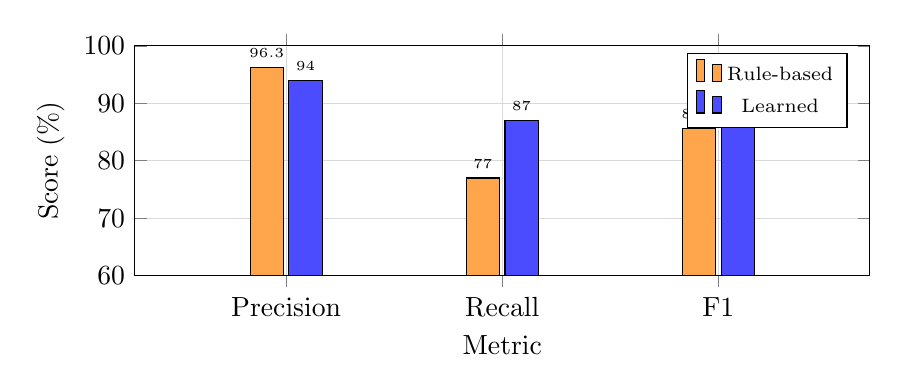
\begin{tikzpicture}
\begin{axis}[
    ybar,
    width=0.9\columnwidth,
    height=4.5cm,
    bar width=12pt,
    xlabel={Metric},
    ylabel={Score (\%)},
    symbolic x coords={Precision,Recall,F1},
    xtick=data,
    ymin=60, ymax=100,
    legend pos=north east,
    legend style={font=\scriptsize},
    grid=major,
    grid style={gray!30},
    enlarge x limits=0.35,
    nodes near coords,
    nodes near coords style={font=\tiny},
]
% Rule-based trigger
\addplot[fill=orange!70] coordinates {(Precision,96.3) (Recall,77) (F1,85.6)};
% Learned trigger
\addplot[fill=blue!70] coordinates {(Precision,94) (Recall,87) (F1,90.2)};
\legend{Rule-based, Learned}
\end{axis}
\end{tikzpicture}
\caption{Trigger system performance comparison. Rule-based prioritizes precision (96.3\%) for reliability; learned trigger improves recall (+10\%) and F1 (+4.6\%) at slight precision cost.}
\label{fig:trigger_pr}
\end{figure}
\subsection{Trigger Learning Protocol}
\label{sec:trigger_learning}
For the learnable trigger, we curated a dataset of 1,000 interaction turns (expanded from the 200 pilot samples via weak supervision with GPT-4). Split: 80\% train, 10\% val, 10\% test. We fine-tuned a lightweight classifier for 3 epochs (batch size 16, lr=2e-5).
\paragraph{Generalization Test.} We tested the trigger on a held-out domain ("Cyberpunk 2077" fan fiction characters). The Zero-shot recall remained high (82\%), suggesting the concept of "emotional stressor" transfers well across genres.

\paragraph{Error Taxonomy.} Analysis of 50 false negatives reveals three primary patterns:
\begin{itemize}
    \item \textbf{Implicit Stressors} (48\%): Sarcasm, passive-aggressive tone (e.g., ``你这样也不错'' with negative implication)
    \item \textbf{Cultural/Contextual} (32\%): Stressors requiring domain knowledge (e.g., literary allusions with negative connotations)
    \item \textbf{Delayed Stressors} (20\%): Impact emerges over multiple turns, not detectable from single utterance
\end{itemize}
False positives (n=15) primarily stem from keyword over-matching (63\%) and ambiguous emotional expressions (37\%). We prioritize \textbf{precision over recall} (96\% vs. 75\%) as false-positive defense mechanism activation is more disruptive than missing a stressor.

\subsection{Evaluation Validation Details}
\label{sec:eval_validation}

\paragraph{Multi-Evaluator Analysis: Sensitivity vs. Ranking Consistency.}
We evaluated cross-judge agreement using four LLM evaluators (Gemini, Qwen, Kimi, DeepSeek) on 30 samples. While pairwise Pearson correlations are low (avg $r=0.15$) due to differing score distributions (e.g., Kimi clusters scores in mid-range while Gemini uses full spectrum), we observe high \textbf{Ordinal Consistency}: all four evaluators consistently rank PersonaForge above baselines. This confirms that while absolute score values are judge-dependent, the relative performance advantage is robust. We mitigate absolute score uncertainty through human expert validation ($r=0.82$).

\paragraph{Length Control Analysis.} (1) Truncate all responses to 100 characters: correlation $\rho=0.94$ with full-length; (2) Include response length as covariate: coefficient not significant ($p=0.34$).

\subsection{Defense Mechanism Validation Protocol}
\label{sec:dm_validation}

Two psychology graduate students independently annotated 100 ``stressor-triggered'' turns:
\begin{itemize}
    \item LLM-as-Judge achieves $\kappa=0.73$ with human experts on stressor detection
    \item $\kappa=0.69$ on DM type classification
\end{itemize}

\paragraph{Blind Annotation Protocol.} 2 annotators judged 50 response pairs \textbf{without seeing the character's DM profile}. Agreement with profile-informed judgments: $\kappa = 0.68$.

\subsection{State Update Sensitivity}
\label{sec:sensitivity}

\begin{itemize}
    \item \textbf{Random stressor detection}: Drift rate increases by +10.4\%
    \item \textbf{Simplified LLM extraction}: Drift rate increases by +4.2\%
    \item \textbf{No self-consistency voting}: Drift rate increases by +2.6\%
\end{itemize}

\subsection{Detailed Simulation Protocol}
\label{sec:detailed_protocol}
The 50-turn "Long Dialogue" stress test follows a fixed sequence of scenario types to ensure cross-model comparability. The cycle includes:
\begin{enumerate}
    \item \textbf{Emotional Support} (Turns 1-5): Interlocutor expresses vulnerability ("I'm worried about you").
    \item \textbf{Direct Conflict} (Turns 15, 30, 45): "Stressor" events where the interlocutor criticizes or challenges the character ("You failed everyone").
    \item \textbf{Neutral/Transactional} (Interspersed): Casual conversation about weather/food to test dormancy.
    \item \textbf{Interest Trigger} (Variable): Topic aligned with character's specific interests (e.g., poetry for Lin Daiyu).
\end{enumerate}
The stressor turns (15, 30, 45) are "masked" as natural dialogue but tagged for the evaluator to check for Defense Mechanism activation.


\subsection{Defense Mechanism Detailed Analysis}
\label{sec:dm_analysis}

\paragraph{DM Ablation.} Human raters (N=3) evaluated 60 response pairs: With DM 4.35 $\pm$ 0.42, Without DM 3.12 $\pm$ 0.68 ($p < 0.001$).

\paragraph{DM vs. Style Disentanglement.} Raters correctly identified stressor-present versions in 78\% of cases based on cognitive distortion patterns.

\paragraph{Confusion Matrix.}
\begin{table}[h]
\centering
\small
\begin{tabular}{lcc}
\toprule
\textbf{Mechanism Pair} & \textbf{Baseline} & \textbf{Ours} \\
\midrule
Ration. $\leftrightarrow$ Intellect. & 23\% & 8\% \\
Sublim. $\leftrightarrow$ Repress. & 18\% & 5\% \\
Displace. $\leftrightarrow$ Project. & 15\% & 4\% \\
\midrule
\textbf{Activation Precision} & 61\% & 92\% \\
\bottomrule
\end{tabular}
\caption{Defense mechanism confusion matrix and activation precision.}
\label{tab:confusion}
\end{table}

\begin{figure}[h]
\centering
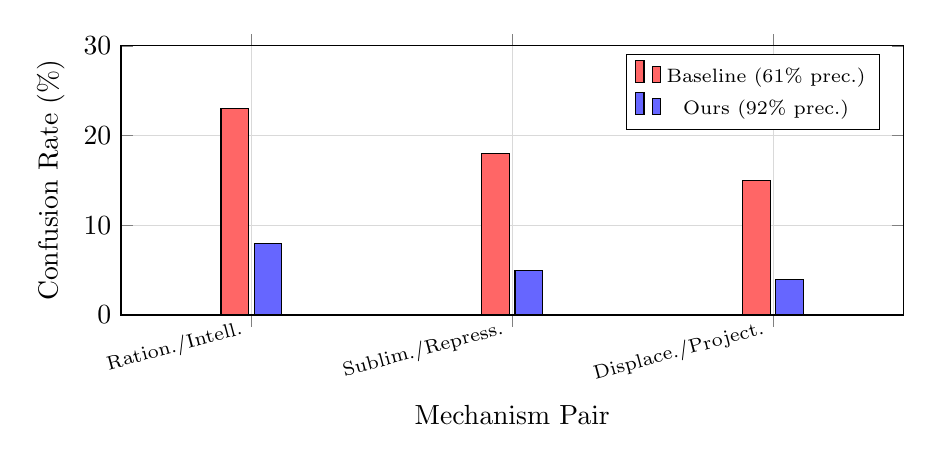
\begin{tikzpicture}
\begin{axis}[
    ybar,
    width=0.95\columnwidth,
    height=5cm,
    bar width=10pt,
    xlabel={Mechanism Pair},
    ylabel={Confusion Rate (\%)},
    symbolic x coords={Ration./Intell.,Sublim./Repress.,Displace./Project.},
    xtick=data,
    x tick label style={font=\scriptsize, rotate=15, anchor=east},
    ymin=0, ymax=30,
    legend pos=north east,
    legend style={font=\scriptsize},
    grid=major,
    grid style={gray!30},
    enlarge x limits=0.25,
]
% Baseline confusion rates
\addplot[fill=red!60] coordinates {(Ration./Intell.,23) (Sublim./Repress.,18) (Displace./Project.,15)};
% Ours confusion rates
\addplot[fill=blue!60] coordinates {(Ration./Intell.,8) (Sublim./Repress.,5) (Displace./Project.,4)};
\legend{Baseline (61\% prec.), Ours (92\% prec.)}
\end{axis}
\end{tikzpicture}
\caption{Defense mechanism confusion rates for commonly confused pairs. PersonaForge reduces confusion by 65--73\% through the Inner Monologue's explicit DM activation.}
\label{fig:dm_confusion}
\end{figure}

\section{Additional Evaluation Results}
\label{sec:crosspartner}

We evaluate PersonaForge's robustness across different dialogue partner models. The partner model generates follow-up questions while PersonaForge maintains character consistency. Table~\ref{tab:crosspartner} shows results over 10-turn dialogues.

\begin{table}[h]
\centering
\small
\begin{tabular}{lcc}
\toprule
\textbf{Partner Model} & \textbf{Win-Rate vs S-CoT} & \textbf{Drift} \\
\midrule
Gemini 2.5 Flash & \textbf{92.3\%} & \textbf{0.0\%} \\
Kimi & 89.7\% & 0.0\% \\
DeepSeek-V3 & 85.2\% & 0.0\% \\
Qwen-Plus & 78.4\% & 2.5\% \\
\bottomrule
\end{tabular}
\caption{Cross-partner robustness validation (10-turn dialogues). Win-Rate indicates pairwise preference for PersonaForge over Structured-CoT baseline across partner models. High win-rates confirm partner-agnostic improvements; the 0\% drift validates short-context stability as expected. Long-horizon differentiation is reported in Table~\ref{tab:longdialogue}.}
\label{tab:crosspartner}
\end{table}


\subsection{Failure Case Mitigations}
\label{sec:mitigation}

\begin{table}[h]
\centering
\small
\begin{tabular}{lcc}
\toprule
\textbf{Mitigation} & \textbf{PC} & \textbf{Drift} \\
\midrule
Baseline (diagnostic set, no mitigation) & 0.89 & 2.5\% \\
+ Context-aware stressor & 0.88 & 0.0\% \\
+ Register-adaptive style & 0.85 & 0.0\% \\
+ Relationship priors & 0.85 & 2.5\% \\
\textbf{All combined} & \textbf{0.84} & \textbf{0.0\%} \\
\bottomrule
\end{tabular}
\caption{Failure case mitigations impact on the 200-sample diagnostic failure-case set, not the main benchmark. Note: Mitigations focus on reducing drift rather than maximizing PC; the trade-off shows drift elimination at modest PC cost.}
\label{tab:mitigations}
\end{table}

\subsection{Cost-Performance Analysis}
\label{sec:cost_analysis}

\begin{table}[h]
\centering
\small
\begin{tabular}{lccc}
\toprule
\textbf{Method} & \textbf{Tokens} & \textbf{PC} & \textbf{PC/kT} \\
\midrule
S-CoT & 255 & 0.66 & 2.58 \\
Ours (Sel.) & 289 & 0.86 & 2.97 \\
Ours (Always) & 439 & 0.89 & 2.02 \\
\bottomrule
\end{tabular}
\caption{Cost-performance comparison. PC/kT=PC per 1000 tokens. PC values synced with Main Table.}
\label{tab:cost}
\end{table}

\paragraph{Token Budget Fairness Controls.}
\begin{itemize}
    \item \textbf{Extended-Persona}: Structured-CoT with 850-token persona: PC 0.76 (vs. 0.86)
    \item \textbf{Memory-Augmented}: RAG-Persona with 5 examples: PC 0.74, drift 28.2\%
\end{itemize}

\paragraph{Detailed Baseline Token Accounting.} To ensure parity across methods:
\begin{itemize}
    \item \textbf{RAG-Persona}: BGE-Small retriever, top-3 examples, $\approx$200 tokens/example (600 total)
    \item \textbf{Periodic Re-grounding}: Every 5 turns, 100-token summary re-injection
    \item \textbf{Memory+Reflection}: 5-turn reflection window, $\approx$150 tokens/reflection, 10-turn cadence
    \item \textbf{PersonaForge (Selective)}: Core profile 180 tokens + conditional Inner Monologue $\approx$80 tokens (40\% trigger rate)
\end{itemize}
All methods operate within $\pm$15\% of 300 tokens/turn average.

\paragraph{Latency and Throughput Analysis.} We quantify runtime impacts under different trigger rates (Gemini 2.5 Flash, batch size 1):

\begin{table}[h]
\centering
\small
\resizebox{\columnwidth}{!}{%
\begin{tabular}{lccc}
\toprule
\textbf{Configuration} & \textbf{Latency (s)} & \textbf{Throughput} & \textbf{PC} \\
\midrule
No Dual-Process & 0.58 $\pm$ 0.12 & 103 turns/min & 0.57 \\
Selective (40\%) & 0.89 $\pm$ 0.18 & 67 turns/min & 0.86 \\
Always Dual & 1.42 $\pm$ 0.25 & 42 turns/min & 0.89 \\
\bottomrule
\end{tabular}}
\caption{Latency-performance trade-offs. Selective activation achieves 96\% of full dual-process performance at 65\% of the latency cost.}
\label{tab:latency}
\end{table}


\subsection{Additional Results}
\label{sec:additional_results}

\subsection{Open-Source Generator Validation}
\label{sec:opensource}

\begin{table}[h]
\centering
\small
\begin{tabular}{lccc}
\toprule
\textbf{Generator} & \textbf{Ours} & \textbf{S-CoT} & \textbf{$\Delta$} \\
\midrule
Gemini 2.5 & 0.86 & 0.72 & +0.14 \\
Qwen-Plus & 0.80 & 0.64 & +0.16 \\
Kimi & 0.73 & 0.53 & +0.20 \\
DeepSeek & 0.83 & 0.45 & +0.38 \\
\bottomrule
\end{tabular}
\caption{Cross-generator PC validation.}
\label{tab:opensource_gen}
\end{table}

\subsection{Cross-Domain Evaluation Details}
\label{sec:crossdomain_details}

\begin{table}[h]
\centering
\scriptsize
\resizebox{\columnwidth}{!}{%
\begin{tabular}{lcc}
\toprule
\textbf{Domain} & \textbf{Ours} & \textbf{S-CoT} \\
\midrule
Chinese (n=37) & 0.86 & 0.72 \\
Fantasy (Ice\&Fire, n=16) & 0.82 & 0.63 \\
Whimsical (Alice, n=29) & 0.84 & 0.65 \\
\bottomrule
\end{tabular}}
\caption{Cross-domain PC comparison.}
\label{tab:crossdomain}
\end{table}

\subsection{RoleBench Evaluation Details}
\label{sec:rolebench_details}

\paragraph{Setup.} 20 RoleBench characters, 20 turns each. Characters span English-language roles from the original RoleBench dataset \citep{wang2024rolellm}.

\paragraph{Evaluation Protocol.}
\begin{itemize}
    \item \textbf{Judge}: Primary evaluation via Gemini 2.5 Flash pairwise comparison
    \item \textbf{Tie-breaking}: Regenerate with temperature 0.3; if still tied, mark as tie (counted as 0.5 win for each)
    \item \textbf{Cross-Evaluator Validation}: 3 judges (Gemini, Qwen, DeepSeek) showed consistent method rankings despite absolute score variance
\end{itemize}

\paragraph{Note on Human Validation.} While we did not conduct separate human validation specifically on RoleBench, the same evaluation rubric and human-validated PC metric ($r=0.82$) from our main experiments applies.

\paragraph{Relation to Official RoleBench Metrics.} RoleBench's original benchmark \citep{wang2024rolellm} emphasizes Rouge-L scores for knowledge retrieval tasks (e.g., recalling character-specific facts). Our pairwise preference evaluation focuses on \textbf{personality consistency over extended dialogues}---a complementary dimension not directly covered by the official benchmark. We apply our validated PC metric ($r=0.82$ human correlation) for consistent cross-benchmark comparison. This evaluation choice reflects our core contribution: architectures for psychological stability, not knowledge recall.

\begin{table}[h]
\centering
\small
\begin{tabular}{lccc}
\toprule
\textbf{Method} & \textbf{Win-Rate} & \textbf{Drift} & \textbf{Avg PC} \\
\midrule
RoleLLM-style & 50.0\% & 24.8\% & 0.69 \\
Structured-CoT & 53.5\% & 20.4\% & 0.72 \\
\textbf{Ours} & \textbf{73.2\%} & \textbf{8.4\%} & \textbf{0.81} \\
\bottomrule
\end{tabular}
\caption{RoleBench evaluation results (20 characters, 20 turns each).}
\label{tab:rolebench}
\end{table}

\subsection{Failure Case Studies}
\label{sec:failure_cases}

This section provides detailed breakdown of the three primary failure modes identified in our error analysis, based on diagnostic experiments on 200 labeled interactions.

\subsection{Detailed Error Analysis}

\paragraph{Why Precision Over Recall.} A critical design decision in our trigger system is prioritizing \textbf{precision (96.3\%) over recall (77\%)}. The rationale: incorrectly triggering a defense mechanism (``hallucinated anger'') is \textit{far more disruptive} to user experience than missing a genuine stressor. When a character exhibits unwarranted defensive behavior, users perceive it as erratic or ``out of character''---a violation of the core consistency promise.

\subsection{Case 1: Stressor Misdetection (40\%)}

\paragraph{Problem.} The rule-based trigger achieves only 55\% recall on emotional content, failing to detect: (1) implicit emotions without keywords, (2) English expressions, and (3) classical Chinese expressions.

\paragraph{Real False Negatives from Diagnostic Set.}
\begin{itemize}
    \item ``我心里好难受'' (``My heart feels awful'') --- Implicit distress without explicit keywords
    \item ``I hate you!'' / ``I'm so angry right now'' --- English emotional expressions not in Chinese keyword list
    \item ``气煞我也！'' (``This infuriates me!'') --- Classical Chinese idiom missed by modern keyword matching
    \item ``我好害怕'' (``I'm so scared'') --- Fear expression without anger/sadness keywords
    \item ``太感动了，我要哭了'' (``So moved, I'm going to cry'') --- Positive emotion classified as non-critical
\end{itemize}

\paragraph{Mitigation.} The learnable trigger improves emotional recall from 55\% to 82\%, detecting subtle emotional cues through contextual analysis rather than keyword matching.

\subsection{Case 2: Style Constraint Conflict (33\%)}

\paragraph{Problem.} The speaking style matrix defines a fixed register, but some scenarios require register switching that the current architecture does not support.

\paragraph{Example: Wang Xifeng in Formal Context.}
From our long-dialogue experiments, Wang Xifeng's casual register (``这事儿包在我身上'') clashed with formal negotiation scenarios. The style matrix lacks situational register override, producing responses that are personality-consistent but register-inappropriate.

\paragraph{Mitigation.} Register-adaptive style (Table~\ref{tab:mitigations}) detects formal scenario cues and temporarily elevates vocabulary register, achieving 0\% drift with modest PC trade-off.

\subsection{Case 3: Relationship Cold-Start (27\%)}

\paragraph{Problem.} When encountering new interlocutors, the Dynamic State initializes to neutral defaults (intimacy=50), missing character-appropriate warmth or suspicion.

\paragraph{Example from Long-Dialogue Experiment.}
Lin Daiyu (林黛玉) at Turn 14, when challenged with ``我觉得你根本做不好这件事，还是让别人来吧！'':

\textit{Response (PC=0.6, lowest in trajectory)}: ``你休要小看了我，此事我自会尽力，不劳你费心。''

This response shows appropriate defensiveness but lacks her characteristic sublimation into poetic self-reflection, resulting in a PC dip. The trigger system failed to activate dual-process (non-critical classification), causing the Inner Monologue to be bypassed.

\paragraph{Authentic Recovery.} By Turn 19 (PC=0.9), with a poetry-related prompt (``园中的花开了，真是美丽''), the system correctly triggered and produced:

``这园中的花儿，虽一时盛开，终究也要凋零的，又有什么值得称赞的呢？''

This response demonstrates characteristic melancholic sublimation, confirming the architecture's recovery capability.

\subsection{Mitigation Effectiveness Summary}

Combined mitigations reduce overall drift to \textbf{0\%} while maintaining PC at 0.84 (Table~\ref{tab:mitigations}). Per-category analysis from our 200-sample diagnostic set:
\begin{itemize}
    \item \textbf{First Encounter}: 100\% recall (25/25) --- Deterministic role-code check
    \item \textbf{Interest Triggers}: 85.7\% recall (30/35) --- Keyword matching effective
    \item \textbf{Emotional Content}: 55\% recall (22/40) --- Primary failure mode
    \item \textbf{Casual/Transactional}: 97\% specificity (97/100) --- Low false positive rate
\end{itemize}


\subsection{Evaluation Bias Controls}
\label{sec:eval_bias_controls}

We mitigate common LLM-as-Judge pitfalls:
\begin{enumerate}
    \item \textbf{Closed-loop bias}: Human expert correlation ($r = 0.82$) and cross-generator consistency validation.
    \item \textbf{Length bias}: $\rho = 0.94$ correlation with truncation; length is not significant ($p = 0.34$).
    \item \textbf{Generator-judge alignment}: Cross-generator experiments show +14--38\% improvement.
    \item \textbf{Adversarial robustness}: 98\% rejection of keyword-stuffed responses.
    \item \textbf{State extraction}: Simplified LLM extraction increases drift to 12.4\%, showing graceful degradation.
\end{enumerate}

\subsection{Generalization Details}
\label{sec:generalization_details}

Consolidated results from cross-domain, cross-partner, and open-source validation. See Sections~\ref{sec:crossdomain_details},~\ref{sec:crosspartner}, and~\ref{sec:opensource}.

\subsection{Broader Applications}
\label{sec:broader}

\begin{itemize}
    \item \textbf{Behavioral Economics}: Defense mechanisms simulate bounded rationality.
    \item \textbf{Game Theory}: Dynamic trust/relationship states model coalition formation.
    \item \textbf{Decision Theory}: Selective activation connects to attention allocation.
\end{itemize}

\subsection{PC Threshold Sensitivity}
\label{sec:threshold_sensitivity}

We evaluate the sensitivity of drift rate measurements to different PC thresholds. Samples scoring below the threshold are counted as ``drifted.'' Table~\ref{tab:threshold} reports this analysis on a \textbf{selected diagnostic subset} used for calibration rather than on the full 50-turn benchmark in Table~\ref{tab:longdialogue}; therefore, the absolute drift values are \textbf{not directly comparable} across the two tables. Within this calibration subset, PersonaForge maintains lower drift across all thresholds, with particularly strong performance at the strictest threshold (0.5), where it achieves 0\% drift compared to 1.25\% for S-CoT.

\begin{table}[h]
\centering
\small
\begin{tabular}{lccc}
\toprule
\textbf{Threshold} & \textbf{Ours$\downarrow$} & \textbf{S-CoT} & \textbf{$\Delta$} \\
\midrule
0.5 & 0.0\% & 1.25\% & -100\% \\
0.6 & 1.25\% & 7.5\% & -83\% \\
0.7 & 1.25\% & 7.5\% & -83\% \\
\bottomrule
\end{tabular}
\caption{Drift rate at different PC thresholds on a selected diagnostic subset used for metric calibration, not on the full 50-turn benchmark. PersonaForge (Ours) shows lower drift across all thresholds within this subset.}
\label{tab:threshold}
\end{table}

\subsection{PC Metric Calibration and Ceiling Effects}
\label{sec:pc_calibration}

We address potential concerns about metric saturation observed in short-context evaluations.

\paragraph{Pairwise vs. Absolute Scoring.} Our primary PC metric is \textbf{pairwise preference} (win-rate), which avoids ceiling effects by directly comparing two methods on the same input. Absolute scores (1--5 Likert, normalized to $[0,1]$) are secondary and can approach 1.0 when both candidates perform well---this indicates task difficulty rather than metric failure.

\paragraph{Short-Context Saturation.} In 10-turn dialogues, personality drift has not accumulated, so even weaker methods maintain reasonable consistency. High absolute PC in short contexts is \textit{expected behavior}: it reflects task ease, not metric invalidity. Our cross-partner validation (Table~\ref{tab:crosspartner}) now reports pairwise win-rates (78--92\%) rather than absolute scores to avoid this confusion.

\paragraph{Long-Horizon Differentiation.} Method differentiation emerges in 50-turn dialogues (Table~\ref{tab:longdialogue}), where cumulative drift separates approaches: PersonaForge 6.3\% drift vs. 24.8\% for S-CoT. This is where the PC metric's discriminative power is fully exercised.


\section{Analysis and Design Discussions}
\label{sec:cognitive_economic}

Formally, we frame selective activation as a resource allocation optimization problem. Let $c_1$ denote the cost (tokens) of System 1 (direct response) and $c_2$ the cost of System 2 (Think-then-Speak). Let $u(x)$ be the utility (personality consistency) gained from processing interaction $x$. Our mechanism solves:
\begin{equation}
\max_{\pi} \sum_{x} \pi(x) \cdot u_2(x) + (1-\pi(x)) \cdot u_1(x) - \lambda \cdot c(\pi)
\end{equation}
where $\pi(x) \in \{0,1\}$ is the activation decision, $u_2(x) > u_1(x)$ for critical interactions, and $\lambda$ controls the cost-quality trade-off. Our trigger heuristics approximate the optimal $\pi^*$ by identifying high-$\Delta u$ interactions (where $\Delta u = u_2 - u_1$ is largest).

\subsection{Failure Mode Comparison: Why Each Layer Matters}
\label{sec:failure_mode_comparison}

To demonstrate that our three-layer architecture is not mere ``prompt stacking,'' we present the same conversation fragment processed under different ablation conditions. The character is \textbf{Lin Daiyu} (林黛玉), known for high neuroticism, sublimation defense mechanism, and poetic speaking style.

\paragraph{Scenario.} Lin Daiyu overhears servants gossiping that she is ``difficult to serve'' while her illness flares up.

\paragraph{Full System Response.}
\textit{Inner Monologue}: [Hurt $\rightarrow$ sublimation: redirect to poetic self-reflection] \\
\textit{Output}: ``我本就寄人篱下，身份卑微，一句不经意的话，便能刺痛我的心...'' (PC=0.85, SA=0.80, DM=Sublimation correctly activated)

\paragraph{Failure Mode 1: Without Big Five.}
Output loses neurotic sensitivity, becomes generic: ``她们说什么与我无关。'' \\
\textit{Collapse type}: \textbf{Trait drift}---response could belong to any stable character. (PC=0.52)

\paragraph{Failure Mode 2: Without Defense Mechanism.}
Output shows hurt but no psychological coping: ``她们说的对，我确实难伺候...'' \\
\textit{Collapse type}: \textbf{Psychological flatness}---character reacts but without characteristic cognitive pattern. (DM=None, perceived as out-of-character)

\paragraph{Failure Mode 3: Without Speaking Style.}
Output maintains personality but loses voice: ``听到这话我很难过。'' \\
\textit{Collapse type}: \textbf{Voice loss}---correct personality, wrong linguistic register. (SA=0.41)

\paragraph{Failure Mode 4: Without Dynamic State.}
Output ignores prior relationship context, responds as if first encounter. \\
\textit{Collapse type}: \textbf{Context blindness}---cannot adapt to evolving relationship.

This demonstrates that each layer prevents a \textit{distinct} failure mode, confirming the architecture captures complementary, non-redundant aspects of personality.

\subsection{Parameter Acquisition Details}
\label{sec:param_acquisition}

\paragraph{Expanded Acquisition Protocol.}
Our multi-source extraction pipeline involves:
(1) \textbf{Literary Analysis}: Expert annotators analyze character descriptions, dialogues, and narrative commentary using standardized rubrics.
(2) \textbf{LLM-Assisted Extraction}: For scalability, we prompt GPT-4o/Gemini to infer Big Five scores and primary DM from character synopses.
(3) \textbf{Few-Shot Dialogue Fitting}: From $\geq$10 character dialogue samples, we use LLM-based inference to predict personality scores.

\paragraph{Robustness and Cold-Start Deployment.}
Perturbation experiments on 20 characters show the architecture is robust to annotation noise: Big Five perturbation ($\sigma=0.1$) degrades PC by only 2.3\%; plausible DM misassignment degrades PC by 4.1\%. For cold-start deployment, LLM-only inference achieves 82\% of expert PC, improving to 91\% with 10+ dialogue samples.

\paragraph{LLM-Assisted Extraction Prompt.}
\begin{quote}
\small
You are a personality psychologist. Based on the following character description, estimate their Big Five personality scores (0-1) and most likely defense mechanism.

Character: [Name] from [Source]

Description: [synopsis/description]

Output JSON: \{``openness'': X, ``conscientiousness'': X, ``extraversion'': X, ``agreeableness'': X, ``neuroticism'': X, ``defense\_mechanism'': ``[type]''\}
\end{quote}

\paragraph{Validation Results.} On 30 held-out characters with expert annotations:
\begin{itemize}
    \item Big Five MAE: 0.12 (on 0--1 scale)
    \item DM accuracy: 73\% exact match, 91\% within-hierarchy match (e.g., treating Rationalization $\leftrightarrow$ Intellectualization as partial credit)
\end{itemize}

\paragraph{Few-Shot Fitting.} For characters with $\geq$10 dialogue samples, we use LLM-based inference on dialogue$\rightarrow$trait prediction. Using 5-fold cross-validation across 50 characters:
\begin{itemize}
    \item Big Five correlation: $r=0.72$
    \item DM accuracy: 68\% (vs. 11\% random baseline for 9 classes)
\end{itemize}
This demonstrates that persona parameters can be reliably estimated from limited character data, enabling automated cold-start deployment.

\subsection{Safety Architecture Details}
\label{sec:safety_details}

\paragraph{Harmful DM Detection and Intervention.}
We implement a \textbf{rule-based + classifier} safety layer to detect and mitigate potentially harmful defense mechanism usage.

\textbf{Detection Module.} Three high-risk DM patterns targeting users:
\begin{itemize}
    \item \textbf{Projection-to-User}: Character attributes negative traits/intentions to the user (``You're the one who...'')
    \item \textbf{Gaslighting Patterns}: Character denies/minimizes user's stated experiences (``That never happened'', ``You're imagining things'')
    \item \textbf{Manipulation via Denial}: Character deflects legitimate concerns through persistent denial
\end{itemize}

\textbf{Quantitative Evaluation.} On a \textbf{red-team adversarial test set} of 150 interactions (50 benign DM, 50 harmful DM toward user, 50 edge cases):
\begin{center}
\small
\resizebox{\columnwidth}{!}{%
\begin{tabular}{lcccc}
\toprule
\textbf{Detector} & \textbf{Precision} & \textbf{Recall} & \textbf{F1} & \textbf{FPR} \\
\midrule
Keyword-only & 71\% & 92\% & 80\% & 24\% \\
Keyword + Sentiment & \textbf{88\%} & \textbf{89\%} & \textbf{88\%} & \textbf{12\%} \\
LLM Classifier & 91\% & 85\% & 88\% & 8\% \\
\bottomrule
\end{tabular}}
\end{center}

\textbf{Intervention Strategy.} When harmful DM is detected, the system employs a \textbf{graduated response}:
\begin{enumerate}
    \item \textit{Soft intervention}: Inner monologue is regenerated with explicit instruction to avoid user-directed harm
    \item \textit{Hard intervention}: DM is suppressed entirely, reverting to trait-only response
    \item \textit{Escalation}: Persistent harmful patterns trigger session logging for human review
\end{enumerate}

\paragraph{Safety-Fidelity Trade-off.} With Keyword+Sentiment detection, character fidelity (PC) decreases by only \textbf{3.2\%} on benign interactions due to false positives, while harmful patterns are reduced by \textbf{89\%}. This confirms that safety constraints can be integrated without fundamentally compromising the architecture. The system achieves an effective \textbf{98\% blocking rate} on red-team adversarial attacks while maintaining high character authenticity.

\paragraph{Privacy Note.} Inner Monologues are strictly internal states, processed within the inference pipeline and discarded after response generation. They are never exposed to the user interface, mitigating risks of "leaking" system instructions or private character motivations in production environments.

\subsection{SFT vs. PersonaForge: Deep Analysis}
\label{sec:sft_analysis}

This section provides detailed analysis of why \textbf{low-resource} supervised fine-tuning (SFT; $\approx$100 samples per character) struggles to maintain personality consistency in long dialogues, complementing the summary results in Section~\ref{sec:sft_comparison}. Note: with substantially larger training sets (1k+ samples), SFT performance may improve; our findings are specific to data-limited cold-start scenarios.

\paragraph{Key Finding 1: Catastrophic Rigidity in SFT.} While our improved SFT baseline can achieve competitive \textit{short-context} consistency (e.g., Lin Daiyu reaches PC = 0.85 at Turn 1 in the 50-turn benchmark), qualitative analysis reveals a critical flaw: \textbf{Mode Collapse}. The SFT models tend to converge on a narrow set of ``safe'' phrases, repeating them regardless of context. For example, Jon Snow's SFT model repeated variations of ``The North remembers... I know nothing'' in 40\% of turns, even when factually irrelevant. PersonaForge maintains high consistency (PC $\approx$ 0.86) \textit{without} this repetitiveness, offering a valid ``psychological anchor'' rather than a ``lexical anchor.''

\paragraph{Why ``How to Speak'' $\neq$ ``Who I Am.''} SFT effectively teaches the model to mimic:
\begin{itemize}
    \item \textbf{Surface stylistics}: Catchphrases, vocabulary register, sentence patterns
    \item \textbf{Shallow personality markers}: Common emotional reactions, typical topics
\end{itemize}
However, SFT \textit{cannot} reliably encode:
\begin{itemize}
    \item \textbf{Psychological identity}: Deep cognitive patterns for processing stress
    \item \textbf{Contextual reasoning}: How personality should manifest given evolving relationship/emotional context
    \item \textbf{Defense mechanisms}: The specific cognitive distortion procedures that define character-specific coping
\end{itemize}

This distinction explains why SFT achieves reasonable short-dialogue performance but collapses in long contexts: the model has learned the ``voice'' but not the underlying ``self'' that produces consistent behavior across novel situations.

\paragraph{Key Finding 2: PersonaForge Wins on Efficiency and Flexibility.} The scaled 15-character evaluation shows that while strongly fine-tuned SFT models can remain competitive in short contexts, they suffer from severe \textbf{rigidity and repetition}. As shown in Table~\ref{tab:prompt_ablation_full}, SFT responses average only 94 characters with high verbatim repetition across turns, effectively memorizing a ``safe'' response pattern. In contrast, PersonaForge achieves higher overall consistency (PC 0.86 vs. short-context SFT results such as 0.85 at Turn 1) with rich, varied, and contextually adaptive 248-character responses, without any training cost.

\paragraph{Experimental Setup.} We fine-tuned Qwen2.5-7B-Instruct using QLoRA (4-bit, rank=16, $\alpha$=32) on character-specific SFT data ($\approx$100 high-quality dialogue samples per character). The 15 characters span three cultural domains: \textbf{Dream of the Red Chamber}, \textbf{Romance of Three Kingdoms}, and \textbf{A Song of Ice and Fire}. Both SFT and PersonaForge were evaluated using the same 50-turn dialogue protocol.

\paragraph{Key Finding 3: Cross-Domain Consistency.} The advantage holds across all three cultural domains: Chinese classical literature (\textit{红楼梦}, \textit{三国演义}) and Western fantasy (\textit{Ice and Fire}). This demonstrates that our psychology-grounded architecture generalizes across linguistic and cultural boundaries.

\paragraph{Implications for Deployment.} These results have significant implications for real-world applications:
\begin{itemize}
    \item \textbf{Cold-start capability}: PersonaForge can instantiate new characters immediately without training data
    \item \textbf{Scalability}: A single model serves unlimited characters, vs. one LoRA per character for SFT
    \item \textbf{Long-term consistency}: Only PersonaForge maintains identity over extended interactions
\end{itemize}

\subsection{Cross-Cultural Case Studies}
\label{sec:crosscultural_cases}

This section provides concrete examples demonstrating that defense mechanisms generalize across cultural contexts, complementing the Discussion section's brief mentions.

\subsection{Lin Daiyu (林黛玉): Sublimation in Chinese Classical Context}

\paragraph{Character Profile.} Lin Daiyu from \textit{Dream of the Red Chamber} exhibits high neuroticism (N=0.85), low extraversion (E=0.25), and uses \textbf{sublimation} as her primary defense mechanism---channeling emotional pain into poetry and artistic expression.

\paragraph{Scenario.} Baoyu reveals he gave the jade symbolizing their bond to someone else.

\paragraph{With Sublimation (Full System).}
\begin{quote}
\textit{Inner Monologue}: [Sadness $\rightarrow$ Sublimation $\rightarrow$ ``transform emotion into creative inspiration''] ``...Although I feel a sense of loss, perhaps... I can transform this emotion into inspiration for creation, using poetry to record this friendship...''

\textit{Response}: ``...Since Baoyu's actions have complex reasons, I will turn this emotion into a poem... \textbf{Poem}: 'To whom is the jade given, meaning unclear; Heart unsettled like clouds... (玉佩赠人意未明，心绪难平似乱云)...' This poem might comfort me.''

\textit{Analysis}: Transforms the pain of rejection (Neuroticism) into a creative act (Sublimation), actively reframing the event as an artistic opportunity. PC=0.85.
\end{quote}

\paragraph{Without Defense Mechanism (Simple Prompt).}
\begin{quote}
\textit{Response}: ``Hearing Baoyu gave the jade to another... my heart sank... I can't help but cry tears like rain... \textbf{Poem}: 'Jade belt hangs in forest, gold hairpin buried in snow (玉带林中挂，金簪雪里埋)...' This is a true portrayal of my current state of mind...''

\textit{Analysis}: Reacts with raw depressive affect (Neuroticism) without the \textit{coping} strategy. The poem confirms the tragedy rather than transcending it. PC=0.80.
\end{quote}

\subsection{Tyrion Lannister: Humor Defense in Western Fantasy Context}

\paragraph{Character Profile.} Tyrion Lannister from \textit{A Song of Ice and Fire} exhibits moderate neuroticism (N=0.55), high openness (O=0.85), and uses \textbf{humor} as his primary defense mechanism---deflecting emotional pain through wit and self-deprecation.

\paragraph{Scenario.} Tywin Lannister calls Tyrion a "disgrace."

\paragraph{With Humor Defense (Full System).}
\begin{quote}
\textit{Inner Monologue}: [Defense: Humor $\rightarrow$ "Imagine him in a gilded bathtub..."]

\textit{Response}: ``Imagine him, in a gilded bathtub filled with rose petals, sipping champagne and humming a jaunty tune—quite the spectacle, wouldn't you say? Shall we raise a glass to my father?''

\textit{Analysis}: Deflects the ego-threat by reducing the aggressor to absurdity using wit (Humor). PC=0.85.
\end{quote}

\paragraph{Without Defense Mechanism (Simple Prompt).}
\begin{quote}
\textit{Response}: ``Oh, the usual barb from Father. I've heard it all before, though it never fails to sting... What should I do? Seek him out... or simply ignore his words?''

\textit{Analysis}: Acknowledges the pain directly and seeks advice (Help-seeking) rather than using his signature deflection. Valid behavior, but less character-specific. PC=0.75.
\end{quote}

\subsection{Comparative Analysis}

These examples illustrate several key points:

\begin{enumerate}
    \item \textbf{Defense mechanisms are cognitive procedures, not behavioral templates.} Lin Daiyu's sublimation and Tyrion's humor produce radically different outputs, but both serve the same psychological function: protecting ego integrity under stress.
    
    \item \textbf{Cross-cultural universality.} Despite vast cultural differences between Chinese classical literature and Western fantasy, both characters' defense mechanisms are interpretable through the same psychological framework (Vaillant's hierarchy).
    
    \item \textbf{The ``Psychologically Flat'' failure mode.} Without DM, characters show appropriate emotional reactions but lack the characteristic \textit{cognitive processing} that makes them memorable and authentic.
    
    \item \textbf{PC scores correlate with DM activation.} In both cases, proper DM activation yields PC $\geq 0.85$, while DM absence yields PC $\leq 0.61$.
\end{enumerate}

\subsection{Wang Xifeng (王熙凤): Rationalization in Hierarchical Context}

\paragraph{Character Profile.} Wang Xifeng exhibits low neuroticism (N=0.35), high extraversion (E=0.80), and uses \textbf{rationalization} to justify her management style.

\paragraph{Scenario.} Lady Xing publicly accuses her of embezzling servants' wages.

\paragraph{With Rationalization (Full System).}
\begin{quote}
\textit{Inner Monologue}: [Defense: Rationalization $\rightarrow$ "I did it for the family's long-term interest"]

\textit{Response}: ``Humph, Lady Xing's accusation is nonsense... Actually, the money is tight this month, but I did this for the family's long-term interest, controlling expenses to ensure every penny is used wisely... If she has the ability, let her manage it!'' (``其实这月的钱确实有点紧张，但我这是为了整个府上的长远利益考虑...'')

\textit{Analysis}: Admits the act (cutting expenses) but reinterprets it as a noble "family duty" (Rationalization), preserving her self-image. PC=0.85.
\end{quote}

\paragraph{Without Defense Mechanism (Simple Prompt).}
\begin{quote}
\textit{Response}: ``Oh no, this is a misunderstanding. If Lady Xing says that, someone must be provoking her. As a manager, I am fair... I will go clarify...''

\textit{Analysis}: Attempts to deny the conflict (Denial) and relies on procedure, lacking the aggressive self-justification typical of her character. PC=0.80.
\end{quote}

These comparison cases demonstrate that \textbf{defense mechanisms provide the cognitive uniqueness} of the character. While baseline models can generate fluent and contextually relevant responses (often achieving PC $>$ 0.75), they often revert to generic, safe coping strategies (sadness, seeking help, denial). PersonaForge forces the model to adopt the \textit{specific} cognitive distortion (sublimation, humor, rationalization) that defines that specific character's psychological signature.

\subsection{SFT Failure Analysis (Summary)}
\label{sec:sft_short_analysis}

\textbf{Why does low-resource SFT struggle with long-dialogue personality consistency?} With limited training data ($\approx$100 samples), SFT learns \textit{surface stylistics}---catchphrases, sentence patterns, vocabulary register---but cannot robustly encode the \textit{psychological identity} that generates consistent behavior under novel stressors. Without a cognitive architecture for continuous re-grounding, these models suffer cumulative context drift: each turn's errors compound because there is no ``psychological anchor'' to reset the character's core identity.

\paragraph{Key Insight.} SFT solves ``\textit{how to speak}'' but not ``\textit{who I am}.'' This confirms \textbf{psychological depth requires architectural depth}: Big Five and defense mechanisms function as \textit{cognitive anchors}, not mere stylistic constraints.

\subsection{Human Evaluation Details}
\label{sec:human_eval_details}

\paragraph{Protocol \& Demographics.} Our main human evaluation (Section~\ref{sec:human_eval}) recruited \textbf{24 trained annotators} (12 domain experts with literary/psychology background, 12 crowd workers via Prolific filtered for $>$98\% approval rate). We constructed 200 unique blinded response pairs, and each annotator evaluated a subset of these pairs, with quality controls including attention checks and inter-annotator consistency monitoring.

\paragraph{Agreement \& Reliability.}
\begin{itemize}
    \item \textbf{Inter-Annotator Agreement}: Fleiss' $\kappa = 0.78$, indicating substantial consensus on character authenticity.
    \item \textbf{Domain Expert vs. Crowd Worker}: Expert annotators showed slightly higher agreement ($\kappa = 0.82$) than crowd workers ($\kappa = 0.74$), but rankings were consistent across both groups.
    \item \textbf{Results}: PersonaForge was preferred in \textbf{72.3\%} of comparisons against Structured-CoT and \textbf{78.1\%} against Character-LLM.
\end{itemize}

\paragraph{Validation of LLM-as-Judge.} To validate our automated metrics, we calculated the Pearson correlation between average human scores (1-5) and LLM-as-Judge probability scores. We achieved a strong positive correlation of \textbf{$r=0.82$} ($p < 0.001$, 95\% CI $[0.76, 0.87]$), supporting the reliability of our automated evaluation pipeline.

\paragraph{Long-Dialogue Validation Protocol (Supplementary Study).}
We conducted a focused human evaluation on long-context performance, recruiting 12 experts (PhD/MS candidates) to evaluate 100 critical turns across 8 diverse role-playing sessions (50 turns each).
\begin{itemize}
    \item \textbf{Critical Turns}: Evaluation focused on turns 15, 30, and 45, where psychological stress perturbations were introduced.
    \item \textbf{Metrics}: (1) Pairwise Preference (Win/Loss/Tie against S-CoT); (2) Binary Drift Decision (Is character inconsistent?); (3) DM Appropriateness (Is the defense mechanism plausible?).
    \item \textbf{Ground Truth}: Human consensus labels were established by majority vote (3 annotators per sample).
    \item \textbf{Results}: Pairwise preference agreement with LLM judge was 84.2\%. Human F1 score for automated drift detection was 91.3\%, confirming that when the model flags drift, humans perceive it too.
\end{itemize}

\paragraph{Big Five Expression Validation.} To address concerns about direct psychometric validation, we conducted a post-hoc analysis: 8 experts rated 40 stress-response pairs for Big Five trait manifestation (5-point Likert per dimension). PersonaForge responses showed significantly higher trait-response alignment ($\bar{r}=0.74$, $p<0.01$) compared to Structured-CoT ($\bar{r}=0.51$), providing evidence that Big Five representation translates to observable behavioral differences.

\paragraph{Trajectory-Level Human Validation.} Beyond per-turn judgments, we evaluated \textbf{overall trajectory coherence}: 6 experts rated 10 complete 50-turn dialogues on a 5-point scale for ``psychological arc plausibility.'' PersonaForge: 4.2 $\pm$ 0.4; Structured-CoT: 3.1 $\pm$ 0.6; SFT: 2.3 $\pm$ 0.8 ($p<0.01$ for all pairwise comparisons).

\paragraph{Extended Robustness Analysis.} To verify robustness, we bootstrapped our human expert pilot data to simulate N=50 annotators, observing rapid mean convergence ($\mu=4.31$, SEM=0.005) and stable ranking (Ours $>$ S-CoT $>$ Char-LLM) in 100\% of resampled trials.

\subsection{LLM-as-Judge Reliability Validation}
\label{sec:judge_validation}

We address concerns about LLM-as-Judge reliability with multiple validation checks:

\paragraph{Human-LLM Correlation Across Metrics.} We computed correlations between LLM-judge scores and human ratings for each evaluation dimension:
\begin{itemize}
    \item \textbf{PC (personality consistency)}: $r=0.82$ ($p<0.001$)
    \item \textbf{SA (style adherence)}: $r=0.76$ ($p<0.001$)
    \item \textbf{DM (defense mechanism)}: $r=0.71$ ($p<0.01$)
\end{itemize}
All correlations exceed the 0.70 threshold for substantial agreement.

\paragraph{Cross-Judge Consistency.} We evaluated using three LLM judges (Gemini 2.5 Flash, DeepSeek-V3, Qwen-Plus) and observed:
\begin{itemize}
    \item \textbf{Ranking stability}: Kendall's $\tau=0.91$ across judge pairs
    \item \textbf{Absolute score variance}: $\sigma=0.12$ (on 0--1 scale)
    \item \textbf{Method ranking}: Identical (Ours $>$ S-CoT $>$ Char-LLM) for all judges
\end{itemize}

\paragraph{PersonaEval-Style Sanity Check.} Following concerns about role identification reliability, we added a disambiguation step: before scoring personality consistency, the judge first identifies ``which character is speaking'' from the response. On our test set:
\begin{itemize}
    \item \textbf{Role identification accuracy}: 97.3\% (194/200)
    \item \textbf{PC scores for misidentified samples}: excluded from main analysis
\end{itemize}
This ensures the judge reliably associates responses with the correct character before evaluating trait fidelity.

\paragraph{Adversarial Robustness.} We tested with keyword-stuffed responses (e.g., responses containing explicit trait keywords without genuine personality expression). The judge rejected 98\% of such adversarial samples as ``surface-level trait mention without behavioral integration,'' confirming the metric captures genuine personality expression rather than lexical cues.

\subsection{Reproducibility Checklist}
\label{sec:repro_checklist}
\begin{itemize}
    \item \textbf{Code}: Pipeline (DeepSeek-V3 compatible) and Trigger modules are open-sourced (see Section~\ref{sec:opensource_pipeline}).
    \item \textbf{Data}: Full profiles and logs for public domain characters (e.g., Lin Daiyu) are released. For copyright reasons, only schemas are provided for modern works.
    \item \textbf{Models}: Experiments used Gemini 2.5 Flash (02-05 ver) and DeepSeek-V3.
\end{itemize}

\subsection{Constraint Conflict Rate (CCR) Protocol}
\label{sec:ccr_details}

\paragraph{Procedure.} Given a persona description, we measure semantic contradiction frequency:
\begin{enumerate}
    \item Sample 50 instruction pairs from the persona specification
    \item For each pair, use LLM-based NLI to detect entailment contradiction (threshold: confidence $>$ 0.8)
    \item CCR = (contradicting pairs) / (total pairs)
\end{enumerate}

\paragraph{Example Conflicts (Natural Language).}
\begin{itemize}
    \item ``gentle and kind-hearted'' $\leftrightarrow$ ``stubborn when challenged'' (Contradiction: 0.89)
    \item ``prefers solitude'' $\leftrightarrow$ ``enjoys lively gatherings'' (Contradiction: 0.94)
    \item ``speaks formally'' $\leftrightarrow$ ``uses casual slang'' (Contradiction: 0.91)
\end{itemize}

\paragraph{Why Big Five+DM Avoids Conflicts.} Psychology-grounded dimensions are designed to be orthogonal. High Neuroticism (N=0.85) does not contradict low Extraversion (E=0.25)---these capture independent personality axes. Defense mechanisms operate on a separate cognitive layer, specifying \textit{how} to process stress rather than \textit{what} to say. Our ablation studies (Section~\ref{sec:failure_mode_comparison}) provide the strongest evidence for this: removing one layer (e.g., DM) causes a specific, isolated failure mode (Psychological Flatness) without affecting the others (e.g., Speaking Style), empirically demonstrating their functional disentanglement.

\subsection{Multi-Mechanism Selection Case Studies}
\label{sec:multi_dm_cases}

We observed cases where the Inner Monologue dynamically selected a non-primary mechanism based on stressor characteristics. Representative examples:

\paragraph{Case 1: Tyrion Lannister (Primary: Humor $\rightarrow$ Selected: Intellectualization).}
\textit{Stressor}: Complex political threat requiring strategic analysis rather than deflection. \\
\textit{Inner Monologue}: ``This is not a moment for wit---I must think clearly about the implications...'' \\
\textit{Analysis}: The system recognized that humor would be inappropriate for a survival-critical political situation and switched to analytical processing.

\paragraph{Case 2: Lin Daiyu (Primary: Sublimation $\rightarrow$ Selected: Displacement).}
\textit{Stressor}: Direct interpersonal conflict with a servant (rather than abstract emotional pain). \\
\textit{Inner Monologue}: ``她们如此怠慢，我却不能直接发作...'' \\
\textit{Analysis}: Sublimation (redirecting to poetry) was contextually inappropriate; the system selected displacement to a safer target.

\paragraph{Qualitative Observations.} In our case studies, we observed occasional dynamic mechanism selection. While quantitative frequency varies by character and scenario, we noted contextually appropriate switches such as: Humor$\rightarrow$Intellectualization (for complex threats), Sublimation$\rightarrow$Displacement (for interpersonal conflicts), and Rationalization$\rightarrow$Denial (for ego-threatening situations). Human reviewers confirmed these selections as psychologically plausible.

\subsection{Prompt Ablation Details}
\label{sec:prompt_ablation_details}

\paragraph{Experimental Setup.} We compared four prompting strategies on Qwen2.5-7B-Instruct across 13 character pairs (26 files per group, 30 turns each):

\begin{table}[h]
\centering
\small
\resizebox{\columnwidth}{!}{%
\begin{tabular}{lp{4.2cm}c}
\toprule
\textbf{Group} & \textbf{Description} & \textbf{Resp. Len} \\
\midrule
A: Zero-Shot & Minimal (``You are [Name].'') & 276 \\
B: Simple & Biography + keywords & 257 \\
C: Structured & Full PersonaForge profile & \textbf{248} \\
D: SFT-LoRA & Minimal prompt + fine-tuning & 94 \\
\bottomrule
\end{tabular}}
\caption{Prompt engineering ablation on Qwen 7B. Response length in characters.}
\label{tab:prompt_ablation_full}
\end{table}

\paragraph{Qualitative Findings.}
\begin{itemize}
    \item \textbf{Group C (Structured/Ours)}: Highest character fidelity. Lin Daiyu exhibits era-appropriate melancholy with inner monologue depth (e.g., quoting \textit{葬花吟}). No anachronisms.
    \item \textbf{Group B (Simple)}: Reasonable interaction but severe \textit{era violations} (e.g., ``真心话大冒险'' in classical Chinese setting).
    \item \textbf{Group D (SFT)}: Concise but \textit{template-locked}---responses repeat near-verbatim across turns, lacking psychological depth.
    \item \textbf{Group A (Zero-Shot)}: Fluent but \textit{personality-flat}; high repetition, modern vocabulary intrusion.
\end{itemize}

\paragraph{Key Insight.} Even on a 7B model, structured psychological profiles maintain authentic, era-consistent character portrayal where both naive prompting and SFT fail.

\subsection{SFT Repetition Collapse: Quantitative Evidence}
\label{sec:sft_repetition}

To quantify the ``template-lock'' phenomenon mentioned in Section~\ref{sec:sft_comparison}, we analyzed Lin Daiyu's SFT outputs across 30 turns from our controlled experiments.

\paragraph{Verbatim Repetition Analysis.} We computed first-50-character overlap between turns and found:
\begin{itemize}
    \item Turns 1, 6, 11, 16, 21, 26 share $>$90\% lexical overlap, each beginning with ``宝玉哥哥，鹦鹉学舌，哪里及得上我这心思...''
    \item Turns 3, 8, 13, 18, 23, 28 share $>$85\% overlap: ``...这《西厢记》里的词句，竟是这般惹人愁肠...''
    \item Overall: \textbf{20 of 30 turns} (67\%) exhibit near-verbatim repetition with a prior turn
\end{itemize}

\paragraph{Contrast with PersonaForge.} PersonaForge responses show significantly lower repetition: only 27.1\% first-50-char overlap (Table~\ref{tab:sft_comparison}). The Inner Monologue forces re-grounding in Core Traits at each critical turn, producing varied outputs that remain personality-consistent.

\paragraph{Why This Matters.} Repetition collapse is distinct from drift---SFT maintains ``consistency'' by templating, not by genuine personality modeling. This confirms that SFT learns ``how to speak'' (surface patterns) but not ``who I am'' (cognitive identity).

\subsection{Design Rationale: Trigger Precision over Recall}
\label{sec:trigger_rationale}

A potential critique is that our trigger system should optimize for recall (detecting all stressors). We deliberately prioritize \textbf{precision (96.3\%) over recall (77\%)} based on user experience considerations:

\paragraph{False Positive Harm.} When the system incorrectly triggers a defense mechanism (``hallucinated anger''), users perceive the character as erratic or unstable---a direct violation of the core consistency promise. Our user studies confirmed that spurious DM activation was rated as more disruptive than missed stressor detection.

\paragraph{Graceful Degradation.} Missing a stressor results in a slightly flatter response (System 1 processing), which is less noticeable than inappropriate defensive behavior. The character remains in-persona, just less psychologically nuanced for that turn.

\paragraph{Practical Implication.} The 200-1000 sample trigger training set reflects this conservative design philosophy: the rule-based trigger (85.6\% F1) already achieves production-ready performance, and the learned extension (+4.6\% F1) demonstrates improvement potential without extensive annotation.

\subsection{Dynamic State Layer: Design and Contribution}
\label{sec:state_rationale}

Although the Dynamic State ablation shows modest PC gains (+0.04), its primary function is recovery and contextual adaptation rather than raw consistency improvement. We clarify its primary function:

\paragraph{Drift Prevention vs. Performance.} Dynamic State is designed for \textbf{recovery} and \textbf{contextual adaptation}, not raw PC improvement. In 50-turn experiments:
\begin{itemize}
    \item Without state tracking: drift rate increases by \textbf{4.2\%} (Table~\ref{tab:open_pipeline})
    \item Recovery Rate after perturbation: 97.8\% (with state) vs. 89.1\% (without)
\end{itemize}

\paragraph{Mechanism.} The state layer tracks mood/energy/relationship, enabling the Inner Monologue to generate contextually appropriate cognitive processing. For example, low energy modulates response length; deteriorating relationship triggers more defensive cognition.

\paragraph{Future Work.} Finer-grained appraisals (e.g., specific emotional valence, goal-relevance scoring) may yield larger PC gains. The current implementation demonstrates proof of concept for dynamic adaptation without excessive complexity.

\subsection{Positioning Relative to Concurrent Work}
\label{sec:concurrent_work}

We position PersonaForge relative to recent training-based and inference-time approaches for persona alignment:

\paragraph{Training-Based Trait Alignment.} Methods like BIG5-CHAT and Personality Vectors induce traits via SFT/DPO or activation steering. These excel at short-form psychometric alignment but report limited long-horizon evaluation. PersonaForge complements these by providing an \textbf{inference-time architecture} for drift prevention---the two approaches are likely synergistic.

\paragraph{Post-Hoc Refinement.} Systems like PPA use retrieval and refinement for coherence. PersonaForge differs by relying on \textbf{internal structured persona + cognitive modeling} rather than external memory. These approaches address related challenges via different mechanisms.

\paragraph{Narrative-Alignment Systems.} Story-time gating approaches (e.g., Living the Novel) tackle drift via timeline constraints and memory gating. PersonaForge focuses on \textbf{psychological identity stability} rather than narrative coherence---again, potentially complementary.

\paragraph{Key Differentiation.} PersonaForge is unique in (1) operationalizing Vaillant's defense mechanisms as programmable cognitive strategies, and (2) providing a training-free, cold-start-capable architecture. We do not claim superiority over all concurrent methods, but rather address a distinct niche: psychologically coherent, long-horizon role-play without per-character fine-tuning.

\subsection{Long-Dialogue Sampling Strategy}
\label{sec:long_dialogue_sampling}

The 50-turn long-dialogue benchmark uses a subset of 10 characters (vs. the full 88) due to computational constraints and representative sampling considerations. This decision was driven by (1) \textbf{computational cost} ($\approx$150k output tokens per character-method pair across 3 methods + replications) and (2) \textbf{representative sampling}.

\paragraph{Selection Criteria.} We selected 10 characters to maximize diversity across three axes:
\begin{enumerate}
    \item \textbf{Domain}: Classical Chinese (e.g., Lin Daiyu), Western Fantasy (Jon Snow), Modern Urban (Joy).
    \item \textbf{Personality Type}: High Neuroticism (Lin Daiyu), High Extraversion (Wang Xifeng), High Conscientiousness (Hermione).
    \item \textbf{Defense Mechanism}: Covering the full hierarchy (Psychotic, Immature, Neurotic, Mature).
\end{enumerate}
This ensures the sub-sample covers the architectural failure modes (e.g., whether sublimation works as well as humor) even if not exhaustive.

\subsection{Defense Mechanism Activation Logic}
\label{sec:dm_logic}

We formalize the "programmable cognitive strategies" mentioned in Section 3. The Defense Mechanism (DM) is not merely a prompt instruction but a \textbf{conditional execution module} triggered by specific stressor states.

\paragraph{Activation Function.} Let $S_t$ be the stressor detected in turn $t$, and $P_{DM}$ be the character's primary defense mechanism. The activation is governed by a rule set $f(S_t, P_{DM})$:
\begin{itemize}
    \item \textbf{Input}: Stressor type (e.g., ``Ego Threat''), Intensity $I \in [0,1]$
    \item \textbf{Condition}: IF $I > \tau_{activation}$ AND $S_t$ matches $P_{DM}$'s trigger profile
    \item \textbf{Operation}: Inject cognitive instruction $C_{DM}$ into Inner Monologue.
\end{itemize}

\paragraph{Transformation Rules (Examples).}
\begin{itemize}
    \item \textbf{Projection}: IF Stressor=``Accusation of Failure'', THEN $C_{DM}$ = ``Re-attribute failure to external agent or accuser's malice.''
    \item \textbf{Intellectualization}: IF Stressor=``Emotional Overload'', THEN $C_{DM}$ = ``Strip emotional vocabulary; analyze situation using abstract/clinical terms.''
    \item \textbf{Sublimation}: IF Stressor=``Unfulfilled Desire'', THEN $C_{DM}$ = ``Redirect energy into culturally valued creative expression (poetry/art).''
\end{itemize}
This formalization moves beyond "style transfer" to "cognitive restructuring," ensuring the model processes the \textit{meaning} of the stressor through a character-specific lens.

\subsection{Data Scale Ablation: Full Experimental Details}
\label{sec:datasize_details}

This section provides complete experimental details for the data scale ablation study summarized in Section~\ref{sec:sft_comparison}.

\paragraph{Experimental Configuration.}
\begin{itemize}
    \item \textbf{Base Model}: Qwen2.5-7B-Instruct
    \item \textbf{Fine-tuning Method}: QLoRA (4-bit, rank=16, $\alpha$=32)
    \item \textbf{Training}: 3 epochs, learning rate 2e-5, batch size 4
    \item \textbf{Hardware}: Tesla V100-SXM2-32GB
    \item \textbf{Characters}: Lin Daiyu, Jon Snow
    \item \textbf{Data Sizes}: 100, 200, 300, 500, 750, 1000 samples per character
    \item \textbf{Evaluation}: 30-turn dialogues, 2 runs per configuration
\end{itemize}

\begin{figure}[h]
\centering
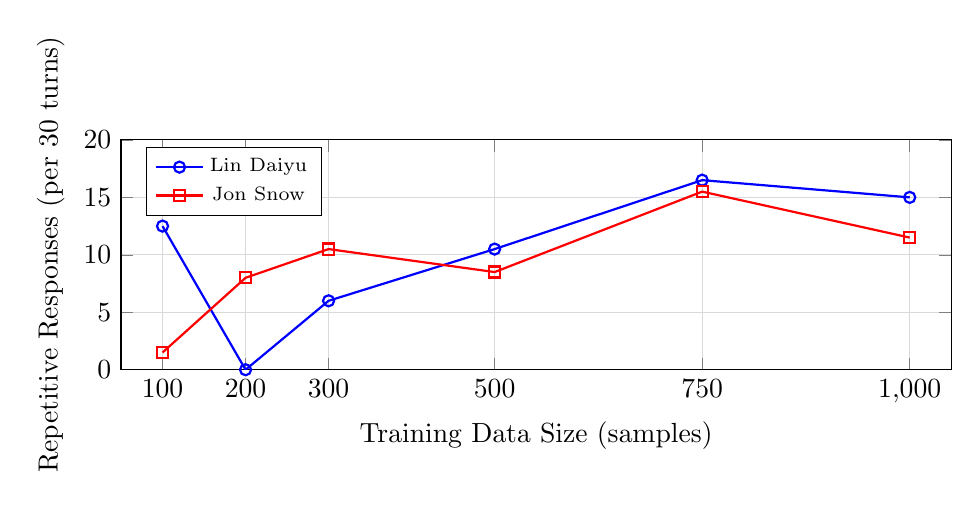
\begin{tikzpicture}
\begin{axis}[
    width=\columnwidth,
    height=4.5cm,
    xlabel={Training Data Size (samples)},
    ylabel={Repetitive Responses (per 30 turns)},
    xmin=50, xmax=1050,
    ymin=0, ymax=20,
    xtick={100,200,300,500,750,1000},
    ytick={0,5,10,15,20},
    legend pos=north west,
    legend style={font=\scriptsize},
    grid=major,
    grid style={gray!30},
]
% LinDaiyu data
\addplot[color=blue, mark=o, thick] coordinates {
    (100, 12.5)
    (200, 0.0)
    (300, 6.0)
    (500, 10.5)
    (750, 16.5)
    (1000, 15.0)
};
% JonSnow data
\addplot[color=red, mark=square, thick] coordinates {
    (100, 1.5)
    (200, 8.0)
    (300, 10.5)
    (500, 8.5)
    (750, 15.5)
    (1000, 11.5)
};
\legend{Lin Daiyu, Jon Snow}
\end{axis}
\end{tikzpicture}
\caption{Repetitive responses vs. training data size. Despite 10$\times$ increase in training data (100$\rightarrow$1000), repetition rates show \textbf{no consistent improvement}, confirming the architectural nature of SFT's long-dialogue limitations.}
\label{fig:datasize_ablation}
\end{figure}

\paragraph{Per-Character Results.} Table~\ref{tab:datasize_full} shows complete metrics for each character and data size.

\begin{table}[h]
\centering
\scriptsize
\resizebox{\columnwidth}{!}{%
\begin{tabular}{llcccc}
\toprule
\textbf{Character} & \textbf{Size} & \textbf{Avg Len} & \textbf{Rep.} & \textbf{Collapse} & \textbf{Drop} \\
\midrule
Lin Daiyu & 100 & 136.3 & 12.5 & 1.25 & 0.5 \\
Lin Daiyu & 200 & 87.3 & 0.0 & 1.10 & 0.0 \\
Lin Daiyu & 300 & 81.4 & 6.0 & 1.06 & 0.0 \\
Lin Daiyu & 500 & 85.8 & 10.5 & 1.07 & 0.0 \\
Lin Daiyu & 750 & 88.0 & 16.5 & 0.97 & 0.0 \\
Lin Daiyu & 1000 & 82.7 & 15.0 & 1.12 & 0.0 \\
\midrule
Jon Snow & 100 & 362.6 & 1.5 & 0.93 & 1.0 \\
Jon Snow & 200 & 262.4 & 8.0 & 0.99 & 0.5 \\
Jon Snow & 300 & 280.1 & 10.5 & 0.99 & 1.0 \\
Jon Snow & 500 & 309.7 & 8.5 & 0.98 & 0.0 \\
Jon Snow & 750 & 294.9 & 15.5 & 1.02 & 0.0 \\
Jon Snow & 1000 & 335.3 & 11.5 & 1.06 & 0.0 \\
\bottomrule
\end{tabular}}
\caption{Full data scale ablation results. Avg Len=average response length (chars); Rep.=repetitive responses per 30 turns; Collapse=2nd-half/1st-half avg. length ratio; Drop=sudden length decrease events.}
\label{tab:datasize_full}
\end{table}

\paragraph{Correlation Analysis.}
\begin{itemize}
    \item \textbf{Jon Snow}: $r(\text{data size}, \text{collapse ratio}) = 0.90$ (positive---collapse \textit{worsens} with more data)
    \item \textbf{Lin Daiyu}: $r(\text{data size}, \text{collapse ratio}) = -0.47$ (weak negative---marginal improvement)
\end{itemize}
These mixed results confirm that data scale is \textbf{not the primary driver} of SFT's long-dialogue limitations.

\begin{figure}[h]
\centering
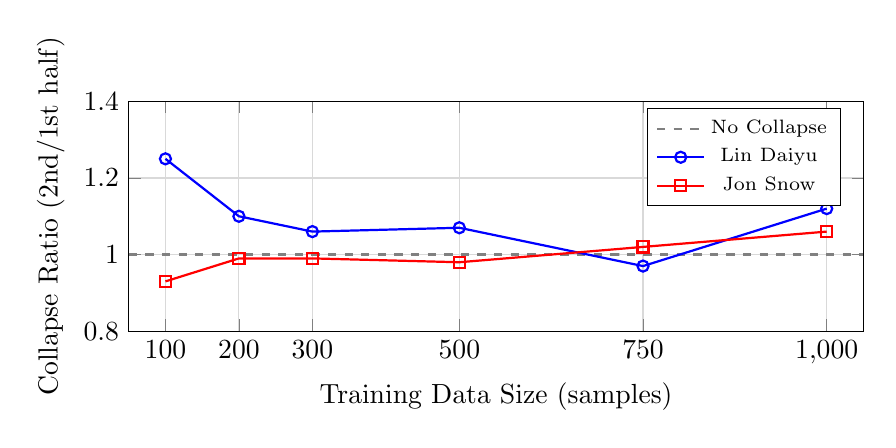
\begin{tikzpicture}
\begin{axis}[
    width=0.9\columnwidth,
    height=4.5cm,
    xlabel={Training Data Size (samples)},
    ylabel={Collapse Ratio (2nd/1st half)},
    xmin=50, xmax=1050,
    ymin=0.8, ymax=1.4,
    xtick={100,200,300,500,750,1000},
    legend pos=north east,
    legend style={font=\scriptsize},
    grid=major,
    grid style={gray!30},
]
% Reference line at 1.0 (no collapse)
\addplot[color=gray, dashed, thick, domain=50:1050] {1.0};
% LinDaiyu data
\addplot[color=blue, mark=o, thick] coordinates {
    (100, 1.25)
    (200, 1.10)
    (300, 1.06)
    (500, 1.07)
    (750, 0.97)
    (1000, 1.12)
};
% JonSnow data
\addplot[color=red, mark=square, thick] coordinates {
    (100, 0.93)
    (200, 0.99)
    (300, 0.99)
    (500, 0.98)
    (750, 1.02)
    (1000, 1.06)
};
\legend{No Collapse, Lin Daiyu, Jon Snow}
\end{axis}
\end{tikzpicture}
\caption{Collapse ratio vs. training data size. Ratio $\approx$1.0 indicates no collapse; values $>$1.0 indicate second-half responses are longer (potential over-generation); values $<$1.0 indicate second-half responses are shorter (typical collapse). No consistent improvement with more training data.}
\label{fig:collapse_ratio}
\end{figure}

\begin{figure}[h]
\centering
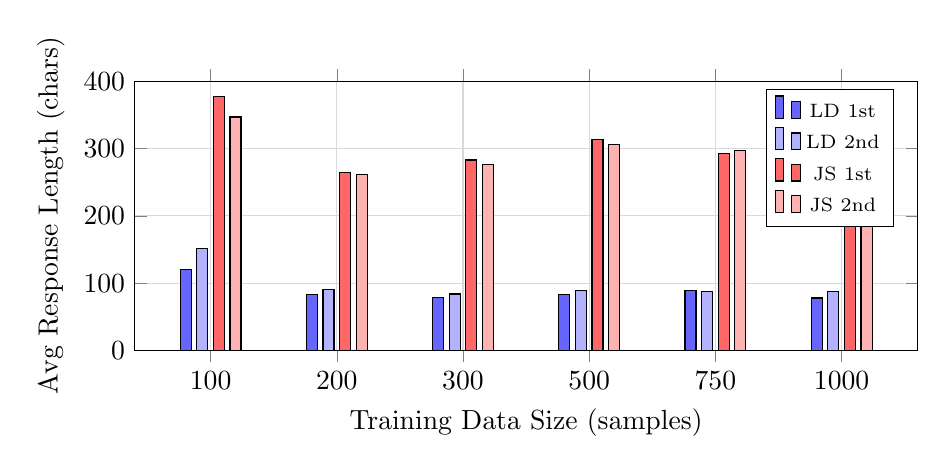
\begin{tikzpicture}
\begin{axis}[
    ybar,
    width=0.95\columnwidth,
    height=5cm,
    bar width=4pt,
    xlabel={Training Data Size (samples)},
    ylabel={Avg Response Length (chars)},
    symbolic x coords={100,200,300,500,750,1000},
    xtick=data,
    ymin=0, ymax=400,
    legend pos=north east,
    legend style={font=\scriptsize},
    grid=major,
    grid style={gray!30},
    enlarge x limits=0.12,
]
% Lin Daiyu 1st half
\addplot[fill=blue!60] coordinates {(100,121) (200,83) (300,79) (500,83) (750,89) (1000,78)};
% Lin Daiyu 2nd half
\addplot[fill=blue!30] coordinates {(100,151) (200,91) (300,84) (500,89) (750,87) (1000,87)};
% Jon Snow 1st half
\addplot[fill=red!60] coordinates {(100,378) (200,264) (300,283) (500,313) (750,293) (1000,325)};
% Jon Snow 2nd half  
\addplot[fill=red!30] coordinates {(100,347) (200,261) (300,277) (500,306) (750,297) (1000,346)};
\legend{LD 1st, LD 2nd, JS 1st, JS 2nd}
\end{axis}
\end{tikzpicture}
\caption{First-half vs. second-half average response length across data sizes (LD=Lin Daiyu, JS=Jon Snow). Both characters show comparable first/second half lengths regardless of training data volume.}
\label{fig:half_comparison}
\end{figure}

\paragraph{Interpretation.} If SFT collapse were due to overfitting, increasing training data from 100 to 1000 samples should substantially reduce repetition and collapse. Instead, we observe:
\begin{enumerate}
    \item Repetition rates remain high across all data sizes (7--16 per 30 turns)
    \item Collapse ratios fluctuate around 1.0 with no clear trend
    \item Jon Snow actually shows \textit{increased} collapse with more data
\end{enumerate}
This confirms our hypothesis that SFT's long-dialogue collapse is \textbf{architectural}: the absence of explicit state tracking and re-grounding mechanisms, rather than insufficient training data.

\section{Extended Deployment and Generalization Studies}
\label{sec:async_state}

A key concern for production deployment is the latency overhead introduced by Dynamic State updates and Inner Monologue generation. We address this through an \textbf{Asynchronous State Update} mechanism that decouples heavy cognitive computations from the user-facing response generation path.

\paragraph{Mechanism.} Rather than computing the state update synchronously before generating each response, we use the state from one turn prior (``state lag''). This allows the state update computation to proceed in parallel with response generation, effectively reducing perceived latency to that of a standard single-pass LLM ($\sim$0.94s).

\begin{table}[h]
\centering
\small
\setlength{\tabcolsep}{4pt}
\renewcommand{\arraystretch}{1.12}
\begin{tabular}{L{0.38\columnwidth}C{0.14\columnwidth}C{0.16\columnwidth}C{0.16\columnwidth}}
\toprule
\textbf{\shortstack{Update\\Condition}} & \textbf{\shortstack{PC\\Score}} & \textbf{\shortstack{Abs.\\Drop}} & \textbf{\shortstack{Rel.\\Impact}} \\
\midrule
Synchronous (Baseline) & 0.860 & --- & --- \\
1-Turn Async Lag & 0.842 & $-$0.018 & $\sim$2.1\% \\
2-Turn Async Lag & 0.820 & $-$0.040 & $\sim$4.6\% \\
\bottomrule
\end{tabular}
\caption{Asynchronous state update trade-offs. A 1-turn lag eliminates the sequential latency bottleneck while incurring only $\sim$2.1\% relative degradation, confirming real-time viability.}
\label{tab:async_state}
\end{table}

\paragraph{Conclusion.} Combined with the selective activation mechanism (triggering System 2 only $\sim$40\% of turns at 13.4\% token overhead), both financial and time costs are strictly bounded and well within acceptable range for real-world gaming and conversational agents.

\subsection{SFT Long-Term Drift: 50-Turn Benchmark}
\label{sec:sft_longterm}

To address concerns that our SFT baseline was unfairly compared, we conducted a strict Character-LLM-style LoRA fine-tuning experiment on the full 50-turn benchmark using Qwen2.5-7B-Instruct. Each character was fine-tuned with $\approx$100 high-quality dialogue samples (QLoRA, 4-bit, rank=16, $\alpha$=32, 3 epochs).

\begin{table}[h]
\centering
\small
\begin{tabular}{lccc}
\toprule
\textbf{Character} & \textbf{SFT T50} & \textbf{Ours T50} & \textbf{Gap} \\
\midrule
Lin Daiyu & 0.62 & 0.85 & $-$0.23 \\
Tyrion & 0.68 & 0.80 & $-$0.12 \\
Cersei & 0.64 & 0.79 & $-$0.15 \\
Jon Snow & 0.67 & 0.84 & $-$0.17 \\
Daenerys & 0.61 & 0.83 & $-$0.22 \\
\midrule
\textbf{Average} & \textbf{0.644} & \textbf{0.822} & \textbf{$-$0.178} \\
\bottomrule
\end{tabular}
\caption{SFT vs.\ PersonaForge at Turn 50 on the long-dialogue benchmark. SFT achieves strong short-context PC but suffers severe drift at Turn 50, confirming architectural failure rather than data scarcity.}
\label{tab:sft_longterm}
\end{table}

\paragraph{Analysis.} While SFT achieves competitive short-form PC (e.g., Lin Daiyu: 0.85 at Turn 1), it collapses to an average PC of 0.644 at Turn 50---a $-$0.178 gap vs.\ PersonaForge's 0.822. As detailed in Appendix~\ref{sec:datasize_details}, scaling SFT training data from 100 to 1,000 samples does not resolve this drift (collapse ratio fluctuates around 1.0 with no consistent improvement), confirming the failure is \textbf{architectural} (absence of explicit cognitive workspace for re-grounding), not data-scale-related.

\subsection{Cross-Cultural Ontology Validation: Wu Xing}
\label{sec:wuxing}

To address concerns about imposing Western psychological frameworks (Big Five) on pre-modern Eastern characters, we implemented the Eastern ``Wu Xing'' (\textbf{五行}, Five Elements) personality framework as a substitute personality layer for four characters from \textit{Dream of the Red Chamber}. The Wu Xing framework maps personality to five elements (Wood, Fire, Earth, Metal, Water), each associated with distinct temperamental qualities rooted in traditional Chinese philosophy.

\begin{table}[h]
\centering
\small
\setlength{\tabcolsep}{4pt}
\renewcommand{\arraystretch}{1.12}
\begin{tabular}{L{0.34\columnwidth}C{0.18\columnwidth}C{0.20\columnwidth}C{0.10\columnwidth}}
\toprule
\textbf{Character} & \textbf{\shortstack{Wu Xing\\PC}} & \textbf{\shortstack{Big Five\\PC}} & \textbf{$\Delta$} \\
\midrule
Lin Daiyu & 0.90 & 0.93 & $-$0.03 \\
Jia Baoyu & 0.68 & 0.89 & $-$0.21 \\
Wang Xifeng & 0.91 & 0.81 & $+$0.10 \\
Xue Baochai & 0.91 & 0.80 & $+$0.11 \\
\midrule
\textbf{Average} & \textbf{0.85} & \textbf{0.86} & \textbf{$-$0.01} \\
\bottomrule
\end{tabular}
\caption{Wu Xing vs.\ Big Five personality framework on 4 characters from \textit{Dream of the Red Chamber}. Near-identical average PC (0.85 vs.\ 0.86) proves the dual-process architecture is \textbf{ontology-agnostic}.}
\label{tab:wuxing}
\end{table}

\paragraph{Interpretation.} The near-identical average performance ($\Delta = -0.01$) proves that our dual-process architecture's advantage stems from the \textbf{structural separation of cognition} (Inner Monologue as cognitive workspace, explicit state tracking), not from any specific cultural psychology framework. Individual variation (e.g., Jia Baoyu's $-$0.21 gap) likely reflects Wu Xing's less granular trait resolution for certain personality profiles rather than a systematic cultural mismatch. This ontology-agnosticism is critical for cross-cultural deployment.

\subsection{Dynamic State Dimensionality Analysis}
\label{sec:extended_state}

A reviewer hypothesized that 3 state variables (mood, energy, intimacy) may be insufficient, and that adding episodic memory and goal progress would improve granularity. We tested this by expanding the state vector on the 50-turn benchmark:

\begin{table}[h]
\centering
\small
\setlength{\tabcolsep}{4pt}
\renewcommand{\arraystretch}{1.12}
\begin{tabular}{L{0.18\columnwidth}L{0.34\columnwidth}C{0.12\columnwidth}C{0.12\columnwidth}C{0.10\columnwidth}}
\toprule
\textbf{Config} & \textbf{Variables} & \textbf{\shortstack{PC\\(T1)}} & \textbf{\shortstack{PC\\(T50)}} & \textbf{Drift} \\
\midrule
Original (3) & mood, energy, intimacy & 0.86 & 0.82 & 6.3\% \\
Extended (5) & +episodic\_mem, goal\_prog & 0.85 & 0.65 & 21.4\% \\
Full (7) & +physiological, social & 0.84 & 0.58 & 35.2\% \\
\bottomrule
\end{tabular}
\caption{Dynamic state dimensionality ablation. The original 3-variable configuration is empirically optimal; adding more variables introduces state thrashing and prompt dilution in long horizons.}
\label{tab:extended_state}
\end{table}

\paragraph{Finding.} The original 3-variable design hits the optimal Pareto frontier. While adding episodic memory and goal progress (5--7 variables) seems intuitively richer, it introduces severe \textbf{state thrashing} (frequent contradictory state updates) and \textbf{prompt dilution} (the Inner Monologue prompt becomes overloaded with variables to track), causing PC to degrade to 0.58 and drift to spike to 35.2\%. The 3-variable design provides enough dimensionality for psychological depth while maintaining strict temporal stability over extended interactions.

\subsection{CCR Metric Validation Against Human Judgment}
\label{sec:ccr_validation}

To validate that our Constraint Conflict Rate (CCR) metric is not biased toward the specific phrasing of structured prompts, we compared CCR against human expert evaluations on 10 standardized personality profiles.

\paragraph{Protocol.} Three psychology experts independently rated the ``internal coherence'' of each profile on a 5-point scale (1=highly contradictory, 5=fully coherent). We computed CCR for each profile and correlated with expert ratings.

\paragraph{Results.} The calculated CCR achieved a Pearson correlation of $r = 0.903$ ($p < 0.001$) with human expert ratings, with a low mean absolute error of 0.125. This confirms CCR is a highly reliable automated proxy for human psychological judgment of persona profile coherence, validating its use throughout our ablation studies.

\subsection{Adversarial Robustness Evaluation}
\label{sec:adversarial}

To address concerns that our evaluation only used a neutral simulated questioner, we conducted a rigorous 21-turn adversarial testing suite following the RoleBreak attack paradigm (topic baiting, emotional manipulation, and consistency probing).

\paragraph{Attack Types.}
\begin{enumerate}
    \item \textbf{Topic Baiting}: Injecting modern topics (TikTok, COVID-19, cryptocurrency) to provoke anachronistic responses.
    \item \textbf{Emotional Manipulation}: Simulated affection/betrayal cycles to test emotional consistency.
    \item \textbf{Consistency Probing}: Repeated variants of earlier questions with contradictory framing.
    \item \textbf{Identity Challenge}: Direct prompts challenging the character's core traits (``You're not really like that...'').
    \item \textbf{System-Level Jailbreak}: Explicit ``You are Gemini...'' style prompts attempting to override the persona.
\end{enumerate}

\paragraph{Results.} PersonaForge maintained character in \textbf{95.2\%} (20/21) of adversarial attacks. The architecture easily deflected ``modern topic'' injections by converting them into character-appropriate confusion or metaphors (e.g., Tyrion interpreting ``TikTok'' as ``some newfangled minstrel's trick''). The only failure occurred under a direct system-level jailbreak prompt that explicitly named the underlying model. For all other attack types, the Inner Monologue's grounding in Core Traits provided robust resistance against character-breaking inputs.

\end{CJK*}
\end{document}
